
Trong chương này, luận văn trình bày kết quả đạt được khi áp dụng kỹ thuật lựa chọn đặc trưng để huấn luyện các mô hình học máy. Bên cạnh đó, quy trình tinh chỉnh siêu tham số bằng tìm kiếm lưới kết hợp kiểm định chéo (cross-validation) cũng được trình bày, cùng với đánh giá kết quả thực nghiệm khi áp dụng các thuật toán học máy như \ac{svm}, \ac{lr}, \ac{nb}, \ac{rf}, \ac{dt}, \ac{gbt}, \ac{xgb} và \ac{mlp} cả trong trường hợp có và không sử dụng kỹ thuật giảm chiều dữ liệu. Ngoài ra, luận văn cũng xác định và trình bày các giá trị tham số tối ưu cho từng thuật toán thông qua phương pháp tìm kiếm theo lưới kết hợp với kiểm định chéo (cross-validation). Dựa trên các kết quả thu được, luận văn sẽ làm rõ vấn đề liệu việc giảm chiều dữ liệu có thực sự cần thiết hay không. Cuối cùng, luận văn đánh giá hiệu quả của các mô hình \ac{el}, sau đó so sánh với các thuật toán học máy truyền thống, từ đó trả lời câu hỏi: \textit{Liệu có nên sử dụng \ac{el} so với các mô hình học máy truyền thống khi làm việc với dữ liệu \ac{iot} hay không?}

\section{Môi trường thực nghiệm}

Việc \emph{huấn luyện} mô hình được thực hiện trên một \textbf{cụm Apache Spark Standalone phân tán} gồm một máy chủ và \textbf{hai thiết bị biên NVIDIA Jetson Orin Nano Super Developer Kit}. Điểm đáng chú ý là cùng một cặp Jetson vừa đóng vai trò \emph{worker} của cụm Spark trong pha huấn luyện, vừa là thiết bị \emph{triển khai} trong pha suy luận thời gian thực (Hình~\ref{fig:ids_diagram}), giúp kiểm chứng tính khả thi của toàn bộ pipeline trên đúng phần cứng mục tiêu.

\begin{itemize}
  \item \textbf{Máy chủ (Spark master):} máy tính xách tay MacBook Air, vi xử lý Apple M3, RAM 16 GB, macOS Sonoma 14.3; đảm nhận điều phối cụm (master), tiền xử lý dữ liệu thô (từ CSV sang Parquet) và chạy hạ tầng Docker (Kafka, PostgreSQL, InfluxDB, Grafana).
  \item \textbf{Hai nút worker:} \textbf{NVIDIA Jetson Orin Nano Super Developer Kit}; cấu hình chi tiết (CPU/GPU/RAM/lưu trữ) nêu tại Bảng~\ref{tab:hardware}, Chương~3; hệ điều hành Ubuntu (NVIDIA JetPack/L4T). Jetson~\#1 đồng thời chạy tiến trình \emph{driver} của Spark (driver là tiến trình điều khiển ứng dụng, khác với vai trò \emph{master} điều phối cụm của MacBook).
  \item {\sloppy \textbf{Phần mềm:} Python 3, Apache Spark / PySpark 3.4.1, MLlib; cấu hình cụm tiêu biểu: \texttt{executor.memory}=3\,GB, \texttt{executor.cores}=4, \texttt{driver.memory}=3\,GB, \texttt{shuffle.partitions}=32; mỗi Jetson được cấp 8\,GB swap trên ổ NVMe để tránh tràn bộ nhớ khi cao điểm (xem \texttt{cluster/spark\_cluster.env}, \texttt{cluster/setup\_swap\_jetson.sh}).\par}
\end{itemize}

Các thuật toán học máy, phương pháp giảm chiều và các bước đánh giá đều được triển khai bằng PySpark và thực thi phân tán trên hai nút Jetson; tập dữ liệu Parquet được đồng bộ sang cả hai worker trước khi huấn luyện. Kiến trúc cụm huấn luyện phân tán (gồm vai trò \textit{master} điều phối trên MacBook và hai \textit{worker}/\textit{executor} trên Jetson) được minh họa ở Hình~\ref{fig:spark_cluster}. Cần phân biệt rõ với Hình~\ref{fig:ids_diagram} (pha suy luận): cùng một cặp Jetson nhưng ở pha huấn luyện đóng vai trò worker của cụm Spark, còn ở pha suy luận đóng vai trò cổng lọc (gate) và bộ phân loại.

Cần nhấn mạnh rằng máy chủ MacBook \emph{chỉ} đảm nhận vai trò \textit{master} điều phối cụm cùng tiền xử lý và hạ tầng dịch vụ, mà \emph{không} tham gia tính toán huấn luyện (không chạy \textit{executor}). Lựa chọn này là có chủ đích: toàn bộ số liệu hiệu năng được báo cáo nhằm phản ánh trung thực khả năng \emph{huấn luyện phân tán ngay trên phần cứng biên} Jetson, đúng với mục tiêu cốt lõi của luận văn. Nếu đưa MacBook (vi xử lý Apple M3, mạnh hơn đáng kể) vào làm nút tính toán, phần lớn khối lượng công việc sẽ dồn về máy chủ, gây mất cân bằng tải (hiện tượng \textit{straggler}) và làm sai lệch các phép đo thời gian/thông lượng, khiến kết quả không còn phản ánh đúng hiệu năng của cụm biên. Vì vậy, cụm đo đạc được giữ \emph{đồng nhất} gồm hai nút Jetson; máy chủ chỉ được dùng để phát triển và kiểm thử nhanh trong giai đoạn xây dựng pipeline.

\begin{figure}[!ht]
    \centering
    \resizebox{\textwidth}{!}{%
    \begin{tikzpicture}[
        font=\small, >=Stealth,
        every node/.style={align=center},
        master/.style={draw=gray!65,        thick, rounded corners, fill=gray!8,   text width=12.6cm, minimum height=1.25cm, inner sep=4pt},
        work/.style  ={draw=accGreen!80!black,  thick, rounded corners, fill=accGreen!8,  text width=5.6cm,  minimum height=2.35cm, inner sep=5pt},
        store/.style ={draw=accBlue,         thick, rounded corners, fill=accBlue!5,   text width=5.6cm,  minimum height=0.85cm, inner sep=3pt},
        lbl/.style   ={font=\footnotesize, fill=white, inner sep=1.5pt, text=gray!35!black},
        dn/.style    ={-{Stealth[length=2.6mm]}, thick, draw=gray!55!black},
        up/.style    ={-{Stealth[length=2.6mm]}, thick, draw=accRed, dashed},
    ]
        \node[master] (m) at (0,0) {\textbf{Máy chủ điều phối: MacBook Air (Apple M3, 16\,GB)}\\[2pt]
            Spark \textbf{Master} (điều phối cụm) \;$|$\; Tiền xử lý CSV\,$\rightarrow$\,Parquet \;$|$\; Docker: Kafka / PostgreSQL / InfluxDB / Grafana\\[1pt]
            \textit{Không chạy executor, không tham gia tính toán huấn luyện}};
        \node[work] (w1) at (-3.6,-4.7) {\textbf{Jetson Orin Nano Super \#1}\\[1pt]
            Spark \textbf{Worker} + \textbf{Driver}\\[2pt]
            Executor: cores=4, mem=3\,GB\\
            Phân vùng dữ liệu (partitions)\\
            swap 8\,GB (NVMe)};
        \node[work] (w2) at ( 3.6,-4.7) {\textbf{Jetson Orin Nano Super \#2}\\[1pt]
            Spark \textbf{Worker}\\[2pt]
            Executor: cores=4, mem=3\,GB\\
            Phân vùng dữ liệu (partitions)\\
            swap 8\,GB (NVMe)};
        \node[store] (s1) at (-3.6,-7.3) {Parquet (đồng bộ)};
        \node[store] (s2) at ( 3.6,-7.3) {Parquet (đồng bộ)};
        \draw[dn] (m.south -| w1) -- node[lbl]{giao tác vụ\\ + partition} (w1.north);
        \draw[dn] (m.south -| w2) -- node[lbl]{giao tác vụ\\ + partition} (w2.north);
        \draw[up] (w1.west) -- ++(-0.75,0) |- (m.west);
        \draw[up] (w2.east) -- ++( 0.75,0) |- (m.east);
        % Nhãn xoay dọc trên đường hồi trái (2 dòng để không lòi lên mũi tên ngang); nền trắng che line
        \node[lbl, rotate=90] at (-7.3,-2.35) {gom kết quả\\(shuffle/collect)};
        \draw[dn] (w1.south) -- (s1.north);
        \draw[dn] (w2.south) -- (s2.north);
    \end{tikzpicture}}
    \caption[Cụm huấn luyện phân tán Apache Spark Standalone]{Cụm huấn luyện phân tán Apache Spark Standalone: máy chủ điều phối (master) và hai Jetson worker/executor}
    \label{fig:spark_cluster}
\end{figure}

\section{Kết quả thực nghiệm}

% Ghi chú: các giá trị trong mục này đã được điền từ loạt chạy leakage-free 2026-07 trên cụm Jetson
% cần điền lại sau khi chạy lại pipeline theo cấu hình đã loại trừ rò rỉ (đã loại
% destination_port và loại bỏ trùng lặp ở mức đặc trưng — xem Chương ref{c:phuongphapthuchien}).
% Các số liệu cũ (gần như tuyệt đối) thu được khi chưa loại rò rỉ và KHÔNG dùng làm kết quả công bố.
% Giá trị điền vào lấy từ các tệp results/*/...csv tương ứng.

\vspace{1em}
Bảng \ref{tab:model_parameters} tóm tắt thiết lập tham số của các mô hình học máy được sử dụng trong nghiên cứu này. Trong đó, \ac{xgb} và MLP được tinh chỉnh bằng Grid Search kết hợp kiểm định chéo (Kịch bản 3); các mô hình còn lại dùng bộ tham số cố định từ trước, lựa chọn dựa trên các nghiên cứu gần đây và thực nghiệm sơ bộ, nhằm bảo đảm khác biệt quan sát được giữa các phương pháp giảm chiều phản ánh đúng phương pháp thay vì mức độ tinh chỉnh riêng từng mô hình.

\begin{table}[htbp]
\centering
\caption{Tham số tối ưu của các mô hình học máy}
\label{tab:model_parameters}
\small
\renewcommand{\arraystretch}{0.9}
\small
\begin{tabular*}{\textwidth}{@{\extracolsep{\fill}}llp{2.2cm}p{5.6cm}@{}}
\toprule
\textbf{Mô hình} & \textbf{Tham số} & \textbf{Giá trị} & \textbf{Ý nghĩa/Mô tả} \\
\midrule
\multirow{3}{*}{Decision Tree}
& maxDepth & 15 & Bắt các mẫu tấn công phức tạp. \\
& impurity & entropy & Tiêu chí chia nhánh tối ưu. \\
& minInstancesPerNode & 5 & Số mẫu tối thiểu tại mỗi nút lá. \\
\midrule
\multirow{4}{*}{Logistic Reg.} & maxIter & 200 & Đảm bảo hội tụ trên tập dữ liệu lớn. \\
& regParam & 0{,}001 & Kiểm soát mức điều chuẩn (regularization). \\
& elasticNetParam & 0{,}0 & Sử dụng Ridge (L2) ổn định hơn. \\
& threshold & 0{,}5 & Ngưỡng quyết định nhị phân. \\
\midrule
\ac{svm} (LinearSVC) & maxIter & 200 & Số lần lặp tối ưu hóa biên. \\
& regParam & 0{,}001 & Tham số điều chuẩn biên quyết định. \\
\midrule
\ac{nb} & modelType & gaussian & Phù hợp cho đặc trưng liên tục. \\
& smoothing & 1{,}0 & Làm mượt Laplace. \\
\midrule
\multirow{3}{*}{Random Forest} 
& numTrees & 200 & Đảm bảo độ ổn định kết quả. \\
& maxDepth & 15 & Chiều sâu tối đa của cây rừng. \\
& featureSubsetStrategy & sqrt & Chọn đặc trưng ngẫu nhiên mỗi nút. \\
\midrule
\multirow{4}{*}{\ac{gbt}}
& maxIter & 150 & Số vòng boosting tối đa. \\
& maxDepth & 6 & Chiều sâu của các cây yếu. \\
& stepSize & 0{,}05 & Tốc độ học (learning rate) của boosting. \\
& subsamplingRate & 0{,}8 & Tỉ lệ lấy mẫu dữ liệu mỗi vòng boosting. \\
\midrule
\multirow{5}{*}{\ac{xgb}}
& n\_estimators & 300 & Số lượng cây boost trong mô hình. \\
& max\_depth & 8 & Chiều sâu tối đa mỗi cây. \\
& learning\_rate & 0{,}05 & Kiểm soát mức độ học của cây mới. \\
& subsample & 0{,}8 & Tỉ lệ lấy mẫu dữ liệu mỗi cây. \\
& colsample\_bytree & 0{,}8 & Tỉ lệ lấy mẫu đặc trưng mỗi cây. \\
\midrule
\multirow{3}{*}{MLP}
& layers & [$d$, 64, 32, 2] & Mạng nơ-ron 2 lớp ẩn ($d$ = số đặc trưng đầu vào). \\
& maxIter & 150 & Số vòng lặp huấn luyện tối đa. \\
& stepSize & 0{,}01 & Tốc độ học của mạng nơ-ron. \\
\bottomrule
\end{tabular*}
\end{table}

\clearpage
\subsection{Kịch bản 1: Đánh giá hiệu năng cơ sở (Baseline)}
Trong kịch bản này, toàn bộ tập đặc trưng số (khoảng 78 đặc trưng trước khi loại cổng; số chính xác sau khi loại \texttt{destination\_port}/\texttt{source\_port} là 77) được đưa vào mô hình mà chưa qua bất kỳ bước lựa chọn đặc trưng hay giảm chiều nào. Mục tiêu là thiết lập một mức hiệu năng tham chiếu cho các thử nghiệm tiếp theo.

Kết quả hiệu năng của các thuật toán \ac{ml} đơn lẻ và phương pháp Ensemble được trình bày trong Bảng \ref{tab:exp0_ml_metrics}.
\begin{table}[htbp]
\centering
\caption[Hiệu năng phân loại kịch bản Baseline]{Kết quả hiệu năng phân loại kịch bản Baseline (toàn bộ đặc trưng số, $\approx$78 trước khi loại cổng)}
\label{tab:exp0_ml_metrics}
\small
\begin{tabular*}{\textwidth}{@{\extracolsep{\fill}}lcccccc@{}}
\toprule
\textbf{Thuật toán} & \textbf{Accuracy} & \textbf{Precision} & \textbf{Recall} & \textbf{F1-Score} & \textbf{AUC-ROC} & \textbf{AUC-\ac{pr}} \\ 
\midrule
Decision Tree          & 0{,}9986 & 0{,}9925 & 0{,}9983 & 0{,}9954 & 0{,}9994 & 0{,}9988 \\
Logistic Regression    & 0{,}9288 & 0{,}6937 & 0{,}9422 & 0{,}7991 & 0{,}9859 & 0{,}9509 \\
\ac{svm} (LinearSVC)        & 0{,}9199 & 0{,}6650 & 0{,}9395 & 0{,}7788 & 0{,}9843 & 0{,}9485 \\
\ac{nb}            & 0{,}3163 & 0{,}1793 & 0{,}9933 & 0{,}3038 & 0{,}8829 & 0{,}6364 \\
Random Forest          & 0{,}9985 & 0{,}9939 & 0{,}9960 & 0{,}9949 & 0{,}9999 & 0{,}9997 \\
\ac{gbt}                    & 0{,}9980 & 0{,}9900 & 0{,}9965 & 0{,}9932 & 0{,}9998 & 0{,}9991 \\
\ac{xgb}                & 0{,}9991 & 0{,}9950 & 0{,}9993 & 0{,}9971 & 1{,}0000 & 0{,}9999 \\
MLP                    & 0{,}9900 & 0{,}9844 & 0{,}9487 & 0{,}9662 & 0{,}9984 & 0{,}9936 \\
\midrule
\textbf{Hybrid Bagging}   & 0{,}9990 & 0{,}9950 & 0{,}9984 & 0{,}9967 & 1{,}0000 & 0{,}9999 \\
\textbf{Soft Voting}  & 0{,}9991 & 0{,}9952 & 0{,}9985 & 0{,}9969 & 1{,}0000 & 0{,}9999 \\
\bottomrule
\end{tabular*}
\end{table}

% (Ghi chú nội bộ: điền số liệu từ results/ml_01_baseline/ và ml_07_cross_method_comparison/cross_method_summary.csv sau khi chạy pipeline loại trừ rò rỉ.)
Với cấu hình đã loại trừ rò rỉ dữ liệu, nhóm mô hình dựa trên cây (Random Forest, \ac{xgb}, GBT) được kỳ vọng dẫn đầu, với F1 thấp hơn mức gần-tuyệt-đối của các cấu hình có rò rỉ và phản ánh đúng độ khó thực của bài toán; kết luận ``mô hình nào tốt nhất'' chỉ được đưa ra khi chênh lệch vượt khoảng tin cậy (xem mục kiểm định thống kê). Do dữ liệu mất cân bằng mạnh, AUC-PR và recall trên lớp tấn công được ưu tiên hơn Accuracy khi diễn giải, vì Accuracy có thể gây lạc quan giả tạo (một mô hình luôn đoán lớp benign chiếm đa số vẫn đạt Accuracy cao).

\subsection{Kịch bản 2: So sánh chiến lược giảm chiều dữ liệu}
Chúng tôi thực hiện so sánh 3 chiến lược chính nhằm giảm số lượng đặc trưng nhưng vẫn đảm bảo hiệu năng:
\begin{enumerate}
    \item \textbf{\ac{rf} Feature Importance}: Trích xuất 30 đặc trưng có điểm số quan trọng cao nhất từ Random Forest.
    \item \textbf{\ac{shap} Importance}: Sử dụng giá trị Shapley từ mô hình \ac{xgb} để chọn ra 30 đặc trưng có ảnh hưởng lớn nhất.
    \item \textbf{\ac{pca} (k=40)}: Giảm chiều dữ liệu từ không gian đặc trưng gốc ($\approx$78 chiều trước khi loại cổng) xuống 40 thành phần chính.
\end{enumerate}

\noindent Lưu ý rằng \ac{pca} dùng $k=40$ --- nhiều hơn 30 đặc trưng của \ac{rf}/\ac{shap}, vì đây là phép \emph{trích xuất} chứ không phải \emph{chọn lọc}: mỗi thành phần chính chỉ là một tổ hợp tuyến tính mang một phần phương sai, nên cần nhiều thành phần hơn để giữ lượng thông tin (phương sai tích lũy) tương đương với tập 30 đặc trưng gốc. Trong dải quét chung $\{20,30,40\}$, $k=40$ là mức giữ phương sai cao nhất, nên là điểm vận hành đại diện công bằng nhất cho \ac{pca}; ép $k=30$ sẽ làm \ac{pca} mất thêm phương sai và bất lợi khi so sánh.

Bảng \ref{tab:summary_comparison} tóm tắt sự khác biệt giữa các phương pháp. Mô hình đại diện (cột \emph{Mô hình tốt nhất}) của mỗi phương pháp được chọn theo F1 trên tập kiểm định (validation) tách từ tập huấn luyện; tập kiểm tra không tham gia khâu chọn lọc này. Mục tiêu là kiểm chứng giả thuyết: lựa chọn đặc trưng (\ac{rf}/\ac{shap} Top-30) giữ được hiệu năng gần với baseline trong khi giảm hơn 60\% số đặc trưng, qua đó phù hợp cho triển khai biên.

\begin{table}[htbp]
\centering
\caption[So sánh hiệu năng tốt nhất của các phương pháp giảm chiều]{So sánh hiệu năng tốt nhất của các phương pháp lựa chọn đặc trưng và giảm chiều}
\label{tab:summary_comparison}
\small
\begin{tabular*}{\textwidth}{@{\extracolsep{\fill}}lccccc@{}}
\toprule
\textbf{Phương pháp} & \textbf{\shortstack{Số đặc\\trưng}} & \textbf{\shortstack{Mô hình\\tốt nhất}} & \textbf{F1-Score} & \textbf{\shortstack{Huấn luyện\\(s)}} & \textbf{\shortstack{Dung lượng\\(MB)}} \\ \midrule
Baseline (Toàn bộ) & 77 & \ac{xgb} & 0{,}9971 & 4615{,}5 & 2{,}32 \\
\ac{rf} Importance & 30 & \ac{xgb} & 0{,}9922 & 1295{,}1 & 2{,}52 \\
\ac{shap} Importance & 30 & \ac{xgb} & 0{,}9970 & 1226{,}1 & 0{,}003$^{\dagger}$ \\
\ac{pca} (k=40) & 40 & \ac{xgb} & 0{,}9939 & 1444{,}8 & 3{,}82 \\ \bottomrule
\end{tabular*}

\tabnote{Baseline dùng toàn bộ 77 đặc trưng số ($\approx$78 trước khi loại cổng). $^{\dagger}$Kích thước đo bằng cách tuần tự hóa mô hình \emph{trên cụm huấn luyện phân tán}: bước lưu mô hình phân tán ghi các phân vùng dữ liệu rừng cây trên executor đang giữ chúng, nên giá trị cỡ KB chỉ bắt được metadata cục bộ trên driver và \emph{thấp hơn thực tế}. Vì dung lượng ensemble cây phụ thuộc số cây và số nút (không phụ thuộc số đặc trưng đầu vào), mô hình \ac{xgb} SHAP Top-30 thực tế tương đương bản RF Top-30 ($\approx$2,5\,MB). Cũng vì vậy, tập đặc trưng rút gọn có thể cho mô hình \emph{lớn hơn} baseline một chút (2,52 so với 2,32\,MB): ít ứng viên tách hơn khiến cây cần nhiều nút hơn để đạt cùng độ tinh khiết. Phép đo tin cậy là bản mô hình xuất ra ở chế độ đơn nút của pipeline triển khai (Mục kết quả biên).}
\end{table}

Ngoài ra, sự so sánh trực tiếp giữa hai phương pháp lựa chọn đặc trưng dựa trên độ quan trọng của \ac{rf} và \ac{shap} được trình bày chi tiết trong Bảng \ref{tab:rf_vs_shap}.

\begin{table}[htbp]
\centering
\caption[So sánh lựa chọn đặc trưng: RF Importance vs SHAP (Top-30)]{So sánh hiệu năng lựa chọn đặc trưng: \ac{rf} Importance vs \ac{shap} Importance (Top-30)}
\label{tab:rf_vs_shap}
\begin{tabular*}{\textwidth}{@{\extracolsep{\fill}}lccc@{}}
\toprule
\textbf{Thuật toán} & \textbf{F1 (\ac{rf} Top-30)} & \textbf{F1 (\ac{shap} Top-30)} & \textbf{Chênh lệch tương đối (\%)} \\ \midrule
Random Forest & 0{,}9879 & 0{,}9955 & +0{,}77 \\
\ac{xgb} & 0{,}9922 & 0{,}9970 & +0{,}48 \\
\ac{gbt} & 0{,}9844 & 0{,}9918 & +0{,}75 \\
Decision Tree & 0{,}9835 & 0{,}9948 & +1{,}15 \\ \bottomrule
\end{tabular*}
\end{table}

\subsection{Kịch bản 3: Tối ưu hóa tham số}
Sau khi chọn được bộ đặc trưng tối ưu từ \ac{shap}, bốn mô hình Spark ML gốc (Random Forest, Decision Tree, \ac{gbt}, Logistic Regression) được tinh chỉnh tham số thông qua Grid Search kết hợp Cross-validation trên tập đặc trưng SHAP Top-30; các mô hình còn lại (\ac{xgb}, MLP, \ac{svm}, \ac{nb}) giữ nguyên bộ tham số cố định ở Bảng~\ref{tab:model_parameters} (xem lý do ở đầu mục).
Việc tinh chỉnh giúp các mô hình cây đạt F1 quanh mức 0,995 (Bảng~\ref{tab:exp2_ml_metrics}); mức cải thiện so với cấu hình cố định là nhỏ do bài toán nhị phân trong-miền đã gần bão hòa, phù hợp với nhận định ở mục kiểm định thống kê.

Kết quả hiệu năng của phương pháp Tối ưu hóa tham số được trình bày trong Bảng \ref{tab:exp2_ml_metrics}.
\begin{table}[htbp]
\centering
\caption{Kết quả hiệu năng phân loại kịch bản Tối ưu hóa tham số}
\label{tab:exp2_ml_metrics}
\small
\begin{tabular*}{\textwidth}{@{\extracolsep{\fill}}lcccccc@{}}
\toprule
\textbf{Thuật toán} & \textbf{Accuracy} & \textbf{Precision} & \textbf{Recall} & \textbf{F1-Score} & \textbf{AUC-ROC} & \textbf{AUC-\ac{pr}} \\ 
\midrule
Decision Tree          & 0{,}9987 & 0{,}9977 & 0{,}9936 & 0{,}9957 & 0{,}9994 & 0{,}9980 \\
Logistic Regression    & 0{,}9541 & 0{,}9787 & 0{,}7094 & 0{,}8226 & 0{,}9749 & 0{,}9371 \\
\ac{svm} (LinearSVC)        & \multicolumn{6}{c}{giữ cấu hình cố định (xem Bảng~\ref{tab:exp0_ml_metrics})} \\
\ac{nb}            & \multicolumn{6}{c}{giữ cấu hình cố định (xem Bảng~\ref{tab:exp0_ml_metrics})} \\
Random Forest          & 0{,}9986 & 0{,}9985 & 0{,}9922 & 0{,}9953 & 0{,}9999 & 0{,}9997 \\
\ac{gbt}                    & 0{,}9985 & 0{,}9979 & 0{,}9924 & 0{,}9951 & 0{,}9999 & 0{,}9993 \\
\ac{xgb}                & \multicolumn{6}{c}{giữ cấu hình cố định (xem Bảng~\ref{tab:exp0_ml_metrics})} \\
MLP                    & \multicolumn{6}{c}{giữ cấu hình cố định (xem Bảng~\ref{tab:exp0_ml_metrics})} \\
\midrule
\textbf{Hybrid Bagging}   & 0{,}9986 & 0{,}9956 & 0{,}9949 & 0{,}9953 & 0{,}9999 & 0{,}9998 \\
\textbf{Soft Voting}  & 0{,}9988 & 0{,}9985 & 0{,}9932 & 0{,}9958 & 1{,}0000 & 0{,}9998 \\
\bottomrule
\end{tabular*}
\end{table}

\subsection{Phân tích khả năng giải thích với \ac{shap}}

Tính giải thích (explainability) là một thành phần thiết yếu trong hệ thống \ac{ids}, nhằm cung cấp cơ sở cho việc xây dựng niềm tin và hỗ trợ vận hành thực tế. Trong nghiên cứu này, phương pháp \ac{shap} (SHapley Additive exPlanations) được sử dụng để phân tích mức độ quan trọng của từng đặc trưng đối với quyết định phân loại của mô hình \ac{xgb}.

\begin{figure}[ht]
    \centering
    \IfFileExists{img/shap_feature_importance_top30.png}{
\includegraphics[width=\linewidth]{img/shap_feature_importance_top30.png}}{\fbox{\parbox{0.9\linewidth}{\centering\vspace{1.4cm}\ph{Biểu đồ SHAP Top-30 --- chạy ml\_06\_feature\_selection\_shap.py rồi \texttt{thesis/collect\_figures.sh}}\vspace{1.4cm}}}}
    \caption[Top 30 đặc trưng quan trọng nhất theo SHAP (mô hình XGBoost)]{Top 30 đặc trưng quan trọng theo giá trị trung bình tuyệt đối SHAP của mô hình \ac{xgb}}
    \label{fig:shap_summary}
\end{figure}

Hình~\ref{fig:shap_summary} xếp hạng 30 đặc trưng quan trọng nhất theo giá trị trung bình tuyệt đối của SHAP (mean $|\text{SHAP}|$): thanh càng dài, đặc trưng càng ảnh hưởng lớn đến quyết định phân loại xét trên toàn bộ mẫu. Để tránh rò rỉ, giá trị SHAP được tính trên một \emph{mẫu phân tầng theo lớp lấy từ tập huấn luyện} (không phải tập kiểm tra); mẫu này được biến đổi qua đúng bộ chuẩn hóa (StandardScaler) đã fit trên tập huấn luyện trước khi tính SHAP, bảo đảm không gian đầu vào của phép giải thích trùng khớp với không gian đầu vào mà mô hình đã học.

\begin{figure}[ht]
    \centering
    \IfFileExists{img/shap_summary_beeswarm.png}{
\includegraphics[width=0.92\linewidth]{img/shap_summary_beeswarm.png}}{\fbox{\parbox{0.9\linewidth}{\centering\vspace{1.4cm}\ph{Biểu đồ SHAP beeswarm --- chạy ml\_06\_feature\_selection\_shap.py rồi \texttt{thesis/collect\_figures.sh}}\vspace{1.4cm}}}}
    \caption[Biểu đồ SHAP Summary (beeswarm)]{Biểu đồ SHAP Summary (beeswarm): phân bố và hướng tác động của từng đặc trưng}
    \label{fig:shap_beeswarm}
\end{figure}

Bổ sung cho xếp hạng tổng thể, Hình~\ref{fig:shap_beeswarm} trình bày biểu đồ SHAP Summary dạng beeswarm: mỗi điểm đại diện cho một quan sát; trục hoành thể hiện giá trị SHAP (dương đẩy dự đoán về lớp tấn công, âm đẩy về lớp bình thường); màu sắc biểu diễn giá trị đặc trưng từ thấp đến cao. Độ phân tán theo trục hoành phản ánh mức độ ảnh hưởng của đặc trưng, độ tập trung thể hiện tính ổn định của tác động.

% (Ghi chú nội bộ: hình và danh sách phải được tạo lại trên tập đặc trưng đã loại rò rỉ;
% điền từ ml_06_feature_selection_shap/shap_feature_importance.csv.)
Bên cạnh đó, giá trị trung bình tuyệt đối của SHAP (mean $|\text{SHAP}|$) được dùng để xếp hạng mức quan trọng tổng thể. Trên tập đặc trưng đã loại trừ rò rỉ, các đặc trưng có mean $|\text{SHAP}|$ lớn nhất là: \texttt{bwd\_packet\_length\_std}, \texttt{init\_win\_bytes\_backward}, \texttt{init\_win\_bytes\_forward} và \texttt{bwd\_packet\_length\_mean}.

Các đặc trưng như \texttt{\path{init_win_bytes_forward}}, \texttt{\path{init_win_bytes_backward}} (kích thước cửa sổ TCP giai đoạn khởi tạo) và \texttt{\path{bwd_packet_length_std}}, \texttt{\path{packet_length_std}} (sự biến thiên độ dài gói tin) phản ánh đặc tính phân phối lưu lượng — là các tín hiệu mạng có ý nghĩa, không phụ thuộc vào định danh dịch vụ. Việc loại \texttt{destination\_port} buộc mô hình dựa vào các đặc trưng hành vi này thay vì ghi nhớ ánh xạ cổng~$\rightarrow$~nhãn.

\subsection{Phân tích rò rỉ dữ liệu (data leakage)}
\label{sec:leakage_analysis}

Đặc trưng \texttt{destination\_port} là một nguồn rò rỉ nhãn tiềm tàng trên CICIDS2017: mỗi loại tấn công được sinh nhằm vào những cổng dịch vụ cố định nên cổng đích tương quan mạnh với nhãn, khiến mô hình dễ ``ghi nhớ'' ánh xạ cổng--nhãn thay vì học hành vi luồng. Engelen và cộng sự~\cite{engelen2021troubleshooting} xếp hiện tượng này vào nhóm \emph{shortcut learning} của CICIDS2017: các thuộc tính định danh (Flow ID, địa chỉ IP, cổng nguồn, nhãn thời gian) phải bị loại khỏi biểu diễn đặc trưng, còn riêng việc dùng cổng đích làm đặc trưng cho \ac{ids} thì các tác giả xem là \emph{còn gây tranh cãi}. Để định lượng ảnh hưởng, luận văn thực hiện phân tích loại bỏ (ablation) giữ/loại cổng với cùng một cấu hình Random Forest cố định a priori (\texttt{numTrees}=200, \texttt{maxDepth}=15, có trọng số lớp; bài toán nhị phân) --- Bảng~\ref{tab:leakage_ablation}. Điều đáng lưu ý là với bài toán \emph{nhị phân trong-miền}, sau khi đã loại trùng lặp luồng ở mức đặc trưng, ảnh hưởng riêng của \texttt{destination\_port} lên F1 chỉ còn \emph{nhỏ} (chênh khoảng $0{,}001$ điểm F1), bởi tác vụ nhị phân trên CICIDS2017 vốn gần mức bão hòa và nguồn rò rỉ \emph{chi phối} (các luồng trùng lặp) đã được xử lý trước bằng bước loại bỏ trùng lặp. Điều này \emph{không} có nghĩa rò rỉ vô hại: giá trị của quy trình loại-trừ-rò-rỉ thể hiện rõ hơn ở đánh giá \emph{đa lớp} với các lớp tấn công hiếm (Mục~\ref{sec:multiclass}) và ở \emph{tổng quát hóa liên bộ dữ liệu} (Mục~\ref{sec:cross-dataset}), nơi các ``lối tắt'' rò rỉ không còn giúp mô hình. Pipeline loại bỏ cả \texttt{destination\_port} lẫn \texttt{source\_port}; phân tích ablation tập trung vào \texttt{destination\_port} vì đây là cổng chi phối.

\begin{table}[htbp]
\centering
\caption[Phân tích loại bỏ (ablation) rò rỉ đặc trưng cổng đích]{Phân tích loại bỏ (ablation) rò rỉ đặc trưng \texttt{destination\_port} với cấu hình Random Forest cố định}
\label{tab:leakage_ablation}
\begin{tabular*}{\textwidth}{@{\extracolsep{\fill}}lccc@{}}
\toprule
\textbf{Cấu hình} & \textbf{F1} & \textbf{Recall (Attack)} & \textbf{AUC-\ac{pr}} \\ \midrule
Giữ \texttt{destination\_port} (rò rỉ) & 0{,}9965 & 0{,}9988 & 0{,}9999 \\
Loại \texttt{destination\_port} (đề xuất) & 0{,}9955 & 0{,}9961 & 0{,}9997 \\ \bottomrule
\end{tabular*}
\end{table}

% (Ghi chú nội bộ: chạy hai lượt — lượt rò rỉ IDS_KEEP_PORT_FEATURES=1 IDS_DEDUP_ON_FEATURES=0
% và lượt đề xuất mặc định — rồi điền Delta F1 vào bảng.)
Cả hai lượt dùng cùng một cấu hình Random Forest cố định từ trước (200 cây, độ sâu 15, trọng số lớp, khớp Bảng~\ref{tab:model_parameters}) để cô lập đúng ảnh hưởng của đặc trưng rò rỉ. Mức chênh lệch F1 giữa hai hàng phản ánh phần hiệu năng bị thổi phồng do đặc trưng rò rỉ; ở đây mức chênh nhỏ vì đã loại trùng lặp trước và tác vụ nhị phân gần bão hòa, nhưng chiều hướng (giữ cổng cho F1/recall cao hơn) vẫn nhất quán với hiện tượng rò rỉ. Mọi kết quả khác trong luận văn dùng cấu hình đã loại cổng.

\subsection{Phân tích hiệu năng hệ thống}
Bên cạnh độ chính xác, hiệu năng hệ thống về thời gian và tài nguyên là yếu tố then chốt cho việc triển khai thực tế.
Kết quả trong Bảng \ref{tab:exp0_system_performance} cho thấy:

\begin{table}[htbp]
\centering
\caption{So sánh thời gian xử lý và kích thước mô hình kịch bản Baseline}
\label{tab:exp0_system_performance}
\small
\begin{tabular*}{\textwidth}{@{\extracolsep{\fill}}lccc@{}}
\toprule
\textbf{Thuật toán} & \textbf{\shortstack{Huấn luyện\\(s)}} & \textbf{\shortstack{Dự đoán\\(s)}} & \textbf{\shortstack{Kích thước\\(MB)}} \\ \midrule
Decision Tree          & 33{,}4   & 6{,}1  & 0{,}0004 \\
Logistic Regression    & 49{,}2   & 5{,}4  & 0{,}009 \\
\ac{svm} (LinearSVC)        & 224{,}3  & 5{,}4  & 0{,}002 \\
\ac{nb}            & 8{,}2    & 5{,}2  & 0{,}012 \\
Random Forest          & 610{,}3  & 18{,}6 & 3{,}69 \\
\ac{gbt}                    & 1346{,}8 & 8{,}9  & 0{,}92 \\
\ac{xgb}                & 4615{,}5 & 9{,}0  & 2{,}32 \\
MLP                    & 314{,}7  & 8{,}0  & 0{,}0004 \\ \midrule
\textbf{Hybrid Bagging}   & 11934{,}5 & 36{,}4 & 7{,}24 \\
\textbf{Soft Voting}  & \textbf{--} & 25{,}6 & \textbf{--} \\ \bottomrule
\end{tabular*}
\end{table}
\begin{itemize}
    \item \textbf{Thời gian huấn luyện}: Các mô hình Gradient Boosting (\ac{gbt}, \ac{xgb}) có thời gian huấn luyện dài nhất nhưng đạt kết quả phân loại cao.
    \item \textbf{Thời gian dự báo}: \ac{xgb} có thời gian dự báo nhanh (khoảng 9 giây cho toàn tập kiểm tra), Random Forest chậm hơn (khoảng 19 giây); cả hai phù hợp cho giám sát theo lô gần thời gian thực.
    \item \textbf{Kích thước mô hình}: các mô hình cây chiếm dung lượng lớn hơn hẳn mô hình tuyến tính (\ac{lr}, \ac{svm}, \ac{nb} chỉ vài KB); \ac{rf} khoảng 3,7 MB và ensemble Hybrid Bagging lớn nhất ($\sim$7,2 MB) do gộp nhiều bộ học cơ sở. \textit{Lưu ý: kích thước được đo bằng cách tuần tự hóa (serialize) \texttt{PipelineModel} của Spark ra đĩa; giá trị này có thể biến thiên theo cách phân mảnh/partition khi lưu nên chỉ mang tính tham khảo tương đối, không dùng làm tiêu chí quyết định lựa chọn mô hình.}
\end{itemize}

\subsection{Kiểm định ý nghĩa thống kê}
\label{sec:stat_validity}
Do các con số F1 giữa những phương pháp/thuật toán hàng đầu rất sát nhau, luận văn không kết luận ``mô hình tốt nhất'' chỉ dựa trên một lần đo. Mô hình đại diện của mỗi phương pháp, cũng như \emph{cặp phương pháp dẫn đầu} được đưa vào kiểm định, đều được chọn theo F1 trên tập kiểm định (validation, 20\% tách từ tập huấn luyện, \texttt{seed}=42); tập kiểm tra không tham gia khâu chọn lọc. Hai phương pháp này sau đó được huấn luyện lại trên $N$ lần \emph{lấy mẫu lại} tập huấn luyện/kiểm tra (mặc định $N{=}6$, ghép cặp trên cùng một phép chia ở mỗi vòng), tính F1 trung bình kèm \emph{hai} loại khoảng tin cậy 95\%: khoảng tin cậy $t$ thông thường và khoảng tin cậy hiệu chỉnh \emph{Nadeau--Bengio}~\cite{nadeau2003inference}, trong đó phương sai nhân hệ số $(1/N + n_{\text{test}}/n_{\text{train}})$ để bù tương quan giữa các lần lấy mẫu lại chồng lấn; khoảng Nadeau--Bengio được dùng làm căn cứ kết luận chính. Ý nghĩa thống kê được kiểm bằng \emph{permutation test ghép cặp hai phía}, \emph{liệt kê đầy đủ} toàn bộ $2^N = 64$ hoán vị đổi dấu (kiểm định chính xác, không xấp xỉ Monte Carlo), do đó $p$ nhỏ nhất khả dĩ là $2/64 \approx 0{,}031$; độ lớn hiệu ứng được báo cáo bằng Cohen's $d$ ghép cặp (Bảng~\ref{tab:stat_validity}). Kết luận: chênh lệch F1 giữa Baseline và \ac{shap} Top-30 \emph{có ý nghĩa thống kê ở mức sàn} ($p \approx 0{,}031$, $d \approx 1{,}94$), nhưng khác biệt tuyệt đối rất nhỏ ($\approx 0{,}0001$ điểm F1) nên hai phương pháp \emph{tương đương về mặt thực dụng}; khi đó tiêu chí phụ (khả năng giải thích, kích thước, chi phí biên) mới là căn cứ lựa chọn. Cần thừa nhận rằng với $N{=}6$, kiểm định có \emph{lực thống kê thấp}; vì vậy một giá trị $p$ không có ý nghĩa tự nó chỉ là bằng chứng yếu cho ``tương đương'', và kết luận được căn cứ đồng thời vào khoảng tin cậy Nadeau--Bengio và Cohen's $d$; tăng $N$ (kèm kiểm định chéo lồng) là hướng củng cố tiếp theo.

\begin{table}[htbp]
\centering
\caption[Độ ổn định qua nhiều lần lấy mẫu và kiểm định ghép cặp]{Độ ổn định qua nhiều lần lấy mẫu và kiểm định ghép cặp (từ \texttt{statistical\_validity\_multiseed.csv})}
\label{tab:stat_validity}
\footnotesize
\begin{tabular*}{\textwidth}{@{\extracolsep{\fill}}llcccc@{}}
\toprule
\textbf{Phương pháp} & \textbf{Mô hình} & \textbf{\shortstack{F1 (mean $\pm$\\CI95 $t$)}} & \textbf{\shortstack{CI95\\Nadeau--Bengio}} & \textbf{\shortstack{$p$\\(ghép cặp)}} & \textbf{Cohen's $d$} \\ \midrule
Baseline (toàn bộ) & \ac{xgb} & 0{,}99734 $\pm$ 0{,}00007 & [0{,}99722; 0{,}99746] & \multirow{2}{*}{0{,}031} & \multirow{2}{*}{1{,}94} \\
\ac{shap} Top-30 & \ac{xgb} & 0{,}99720 $\pm$ 0{,}00009 & [0{,}99705; 0{,}99735] & & \\ \bottomrule
\end{tabular*}
\end{table}

\subsection{Kiểm tra độ ổn định trong-phân-phối}
\label{sec:robustness}
Mô hình đại diện của mỗi phương pháp được đánh giá lại trên một mẫu con của tập kiểm tra (không giao với tập huấn luyện; Bảng~\ref{tab:robustness}). Cần nói rõ: đây chỉ là phép kiểm tra \emph{độ ổn định cùng phân phối} (in-distribution), không phải kiểm thử dịch chuyển phân phối; đánh giá tổng quát hóa thực sự nằm ở thí nghiệm liên bộ dữ liệu (Mục~\ref{sec:cross-dataset}).

\begin{table}[htbp]
\centering
\caption[Kiểm tra độ ổn định trong-phân-phối trên mẫu con tập kiểm tra]{Kiểm tra độ ổn định trong-phân-phối trên mẫu con tập kiểm tra (từ \texttt{robustness\_holdout\_summary.csv})}
\label{tab:robustness}
\begin{tabular*}{\textwidth}{@{\extracolsep{\fill}}llcc@{}}
\toprule
\textbf{Phương pháp} & \textbf{Mô hình} & \textbf{F1 (holdout)} & \textbf{AUC-\ac{pr}} \\ \midrule
Baseline & \ac{xgb} & 0{,}9971 & 0{,}9999 \\
\ac{rf} Top-30 & \ac{xgb} & 0{,}9921 & 0{,}9998 \\
\ac{shap} Top-30 & \ac{xgb} & 0{,}9969 & 0{,}9999 \\
\ac{pca} & \ac{xgb} & 0{,}9939 & 0{,}9998 \\ \bottomrule
\end{tabular*}
\end{table}

\subsubsection{Tổng quát hóa liên bộ dữ liệu}
\label{sec:cross-dataset}
Đánh giá trên tập giữ lại ở trên là phép thử \emph{cùng bộ} (in-domain, cùng phân phối). Để kiểm chứng khả năng \emph{tổng quát hóa} thực sự, mô hình được huấn luyện trên một bộ dữ liệu và kiểm tra trên bộ \emph{khác} (đánh giá \emph{khác bộ}, cross-dataset; và ngược lại) trên tập đặc trưng đã loại trừ rò rỉ \emph{chung} của hai bộ. Do hai bộ dữ liệu đặt tên cột khác nhau (CSE-CIC-IDS2018 dùng tên viết tắt kiểu CICFlowMeter v3), tên cột của CSE-CIC-IDS2018 được ánh xạ về tên chuẩn của CICIDS2017 qua một bảng bí danh (alias) tường minh trong mã nguồn; danh sách đặc trưng chung sau ánh xạ được lưu tại \texttt{common\_features.txt} để bảo đảm tái lập. Mô hình dùng cho thí nghiệm là Random Forest có trọng số lớp (\texttt{weightCol}), nhất quán với cơ chế xử lý mất cân bằng ở Chương~3. Khoảng cách giữa F1 cùng bộ và F1 khác bộ (Bảng~\ref{tab:cross_dataset}) định lượng mức suy giảm khi gặp dịch chuyển phân phối, một thước đo độ ổn định chặt chẽ hơn holdout cùng phân phối.

Do CSE-CIC-IDS2018~\cite{CSECICIDS2018} có quy mô rất lớn ($\sim$16 triệu luồng, $\sim$6\,GB), vượt khả năng xử lý thoải mái của thiết bị biên Jetson (8\,GB), thí nghiệm này dùng \emph{mẫu phân tầng theo nhãn} của CSE-CIC-IDS2018 (tỷ lệ 0{,}2, $\sim$3{,}14 triệu luồng lấy mẫu, còn $\sim$2{,}39 triệu sau khử trùng lặp mức đặc trưng, \texttt{seed}=42, công tắc \texttt{IDS\_SAMPLE\_FRAC}) nhằm bảo toàn tỷ lệ các lớp trong khi vừa với phần cứng; CICIDS2017 dùng $\sim$2{,}23 triệu luồng. Toàn bộ quy trình tiền xử lý và căn chỉnh CSE-CIC-IDS2018 cho thí nghiệm liên bộ dữ liệu được trình bày ở Thuật toán~\ref{alg:prep_2018}; các bước loại trừ rò rỉ (giao đặc trưng chung không chứa cổng/IP, khử trùng lặp mức đặc trưng) hoàn toàn nhất quán với quy trình cho CICIDS2017 (Thuật toán~\ref{data_preparation_ag}). Các con số mẫu được báo cáo tường minh để bảo đảm tính tái lập; việc mở rộng lên toàn bộ CSE-CIC-IDS2018 là hướng phát triển tiếp theo.

\begin{algorithm}[htbp]
\caption{Tiền xử lý và căn chỉnh CSE-CIC-IDS2018 cho đánh giá liên bộ dữ liệu}
\label{alg:prep_2018}
\begin{algorithmic}[1]
\Require Tập tệp CSV của CSE-CIC-IDS2018; lược đồ tên cột chuẩn của CICIDS2017 $\mathcal{S}_{2017}$;
\Statex \qquad bảng bí danh tên cột $\mathcal{A}$ (2018 $\rightarrow$ 2017); tỷ lệ lấy mẫu $r = 0.2$; \texttt{seed} $= 42$
\Ensure Bộ dữ liệu $D_{2018}$ trên tập đặc trưng chung đã loại rò rỉ $\mathcal{F}_{\text{chung}}$, sẵn sàng cho thí nghiệm khác bộ

\State \textbf{Bước 1: Nạp và làm sạch} (giống Thuật toán~\ref{data_preparation_ag})
\State Đọc các tệp CSV; \Call{CleanColumnNames}{}; \Call{HandleInfinityValues}{}; loại null và bản ghi trùng lặp hoàn toàn

\State \textbf{Bước 2: Căn chỉnh tên cột}
\State $\forall c \in \text{columns}(D):\ c \gets \mathcal{A}(c)$ \Comment{ánh xạ tên cột CICFlowMeter v3 về tên chuẩn của CICIDS2017}

\State \textbf{Bước 3: Tạo nhãn nhị phân (không phân biệt hoa/thường)}
\State $y_i \gets 0$ nếu \textsc{lower}(label$_i$) $=$ ``benign'', ngược lại $y_i \gets 1$ \Comment{2018 ghi ``Benign''; so khớp không phân biệt hoa/thường}

\Statex \textcolor{accRed}{\textbf{$\rightarrow$ Loại trừ rò rỉ dữ liệu: Bước 4 và Bước 6}}
\State \textbf{Bước 4 [loại rò rỉ~--~I]: Giao đặc trưng chung, đã loại trừ rò rỉ}
\State $\mathcal{F}_{\text{chung}} \gets (\mathcal{F}_{2017} \cap \mathcal{F}_{2018}) \setminus \mathcal{C}_{\text{exclude}}$ \Comment{$\mathcal{C}_{\text{exclude}}$: destination\_port, source\_port, protocol, IP, timestamp, flow\_id}
\State Lưu $\mathcal{F}_{\text{chung}}$ vào \texttt{common\_features.txt} \Comment{cố định cho cả hai chiều huấn luyện/kiểm tra}

\State \textbf{Bước 5: Lấy mẫu phân tầng theo nhãn}
\State $D \gets \Call{StratifiedSample}{D, r, \text{seed}=42}$ \Comment{bảo toàn tỷ lệ lớp; còn $\sim$3{,}14 triệu luồng}

\State \textbf{Bước 6 [loại rò rỉ~--~II]: Loại trùng lặp ở mức đặc trưng} (tất định, như Bước 4b của Thuật toán~\ref{data_preparation_ag})
\State Gom nhóm theo $\mathcal{F}_{\text{chung}}$; loại toàn bộ nhóm mâu thuẫn nhãn; giữ đúng một đại diện của mỗi nhóm nhất quán \Comment{còn $\sim$2{,}39 triệu luồng}

\State \Return $D_{2018}$ trên tập đặc trưng $\mathcal{F}_{\text{chung}}$
\end{algorithmic}
\end{algorithm}

\begin{table}[htbp]
\centering
\caption[Tổng quát hóa liên bộ dữ liệu CICIDS2017 và CSE-CIC-IDS2018]{Tổng quát hóa liên bộ dữ liệu giữa CICIDS2017 và CSE-CIC-IDS2018}
\label{tab:cross_dataset}
\begin{tabular*}{\textwidth}{@{\extracolsep{\fill}}llcc@{}}
\toprule
\textbf{Huấn luyện} & \textbf{Kiểm tra} & \textbf{Loại} & \textbf{F1} \\ \midrule
CICIDS2017 & CICIDS2017 & cùng bộ & 0{,}9952 \\
CICIDS2017 & CSE-CIC-IDS2018 & khác bộ & 0{,}0423 \\
CSE-CIC-IDS2018 & CSE-CIC-IDS2018 & cùng bộ & 0{,}9245 \\
CSE-CIC-IDS2018 & CICIDS2017 & khác bộ & 0{,}0535 \\ \bottomrule
\end{tabular*}
\end{table}

\textbf{Diễn giải.} Kết quả cho thấy một tương phản rõ rệt và \emph{trung thực}: F1 cùng bộ rất cao ở cả hai chiều (0{,}9952 và 0{,}9245) nhưng F1 khác bộ giảm mạnh xuống 0{,}04--0{,}05, chủ yếu do recall gần bằng không (0{,}022 và 0{,}030) trong khi precision chiều 2017 sang 2018 vẫn đạt 0{,}596, tức mô hình gần như không nhận ra tấn công của bộ dữ liệu kia, chứ không tạo ra cảnh báo sai tràn lan. Nguyên nhân là \emph{dịch chuyển phân phối đặc trưng} giữa hai testbed: khác phiên bản CICFlowMeter (thang đo và cách tính một số đặc trưng thay đổi), khác hạ tầng mạng và cấu hình dịch vụ, khác tổ hợp loại tấn công (HOIC/LOIC-HTTP của 2018 không có trong 2017). Sự sụt giảm này nhất quán với các nghiên cứu cross-dataset trên IDS dựa trên đặc trưng luồng~\cite{dhooge2020interdataset,cantone2024crossdataset,sarhan2022explainable}, và chính là luận cứ mạnh nhất của luận văn: \emph{con số trong-miền gần hoàn hảo (kể cả khi đã loại rò rỉ) không bảo đảm khả năng triển khai sang môi trường khác}; đánh giá liên bộ dữ liệu phải là một phần bắt buộc của quy trình kiểm định IDS~\cite{goldschmidt2025datasets}, và các hướng thích ứng miền (chuẩn hóa theo miền, huấn luyện liên bộ, cập nhật theo drift) là điều kiện tiên quyết cho triển khai thực tế.

\subsection{Đánh giá đa lớp theo loại tấn công}
\label{sec:multiclass}
Phân loại nhị phân (Benign/Attack) trên CICIDS2017 vốn dễ tách; để bộc lộ điểm yếu thực sự, luận văn bổ sung đánh giá \emph{đa lớp theo từng loại tấn công gốc} (precision/recall/F1 từng lớp, macro-F1, weighted-F1 và ma trận nhầm lẫn), gồm lớp Benign và 14 loại tấn công của CICIDS2017. Kết quả cho thấy tương phản rất rõ giữa hai chỉ số tổng hợp: \emph{weighted-F1 $\approx 0{,}998$} (bị chi phối bởi các lớp đa số) nhưng \emph{macro-F1 chỉ $\approx 0{,}806$}, chính là bằng chứng cho thấy độ chính xác nhị phân gần hoàn hảo đã \emph{che giấu} hiệu năng phát hiện kém ở các lớp hiếm. Cụ thể, các lớp đa số (Benign, DoS Hulk, DDoS, PortScan) đạt F1 rất cao ($\geq 0{,}97$), trong khi các lớp cực hiếm suy giảm nghiêm trọng: Web Attack~-- XSS recall chỉ $0{,}027$, Web Attack~-- SQL Injection F1~$=0$ (chỉ 6 mẫu), Bot recall $0{,}46$. Đây là nơi khác biệt giữa các phương pháp lựa chọn đặc trưng thể hiện rõ nhất và cũng là hướng cần cải thiện (xử lý mất cân bằng, tăng cường dữ liệu lớp hiếm). Kết quả chi tiết theo từng lớp được trình bày trong Bảng~\ref{tab:per_class}, và ma trận nhầm lẫn đa lớp tương ứng được minh họa ở Hình~\ref{fig:confusion_matrix}.

\begin{table}[htbp]
\centering
\caption[Hiệu năng theo từng lớp tấn công]{Hiệu năng theo từng lớp tấn công (từ \texttt{per\_class\_metrics.csv})}
\label{tab:per_class}
\small
\begin{tabular*}{\textwidth}{@{\extracolsep{\fill}}lcccc@{}}
\toprule
\textbf{Lớp} & \textbf{Support} & \textbf{Precision} & \textbf{Recall} & \textbf{F1} \\ \midrule
Benign                       & 380.119 & 0{,}9981 & 0{,}9997 & 0{,}9989 \\
DoS Hulk                     & 34.446  & 0{,}9990 & 0{,}9904 & 0{,}9947 \\
DDoS                         & 25.694  & 0{,}9996 & 0{,}9992 & 0{,}9994 \\
DoS GoldenEye                & 2.020   & 1{,}0000 & 0{,}9757 & 0{,}9877 \\
FTP-Patator                  & 1.147   & 0{,}9965 & 0{,}9965 & 0{,}9965 \\
DoS slowloris                & 1.068   & 0{,}9953 & 0{,}9925 & 0{,}9939 \\
DoS Slowhttptest             & 1.023   & 0{,}9286 & 0{,}9912 & 0{,}9589 \\
SSH-Patator                  & 642     & 1{,}0000 & 0{,}9346 & 0{,}9662 \\
PortScan                     & 383     & 1{,}0000 & 0{,}9530 & 0{,}9759 \\
Web Attack~-- Brute Force    & 311     & 0{,}7346 & 0{,}7299 & 0{,}7323 \\
Bot                          & 290     & 1{,}0000 & 0{,}4552 & 0{,}6256 \\
Web Attack~-- XSS            & 111     & 1{,}0000 & 0{,}0270 & 0{,}0526 \\
Infiltration                 & 12      & 1{,}0000 & 0{,}6667 & 0{,}8000 \\
Web Attack~-- SQL Injection  & 6       & 0{,}0000 & 0{,}0000 & 0{,}0000 \\
Heartbleed                   & 3       & 1{,}0000 & 1{,}0000 & 1{,}0000 \\ \midrule
\multicolumn{2}{l}{\textbf{macro-F1 / weighted-F1}} & \multicolumn{3}{c}{0{,}806 / 0{,}998} \\ \bottomrule
\end{tabular*}
\end{table}

\begin{figure}[htbp]
    \centering
    \IfFileExists{img/confusion_matrix.png}{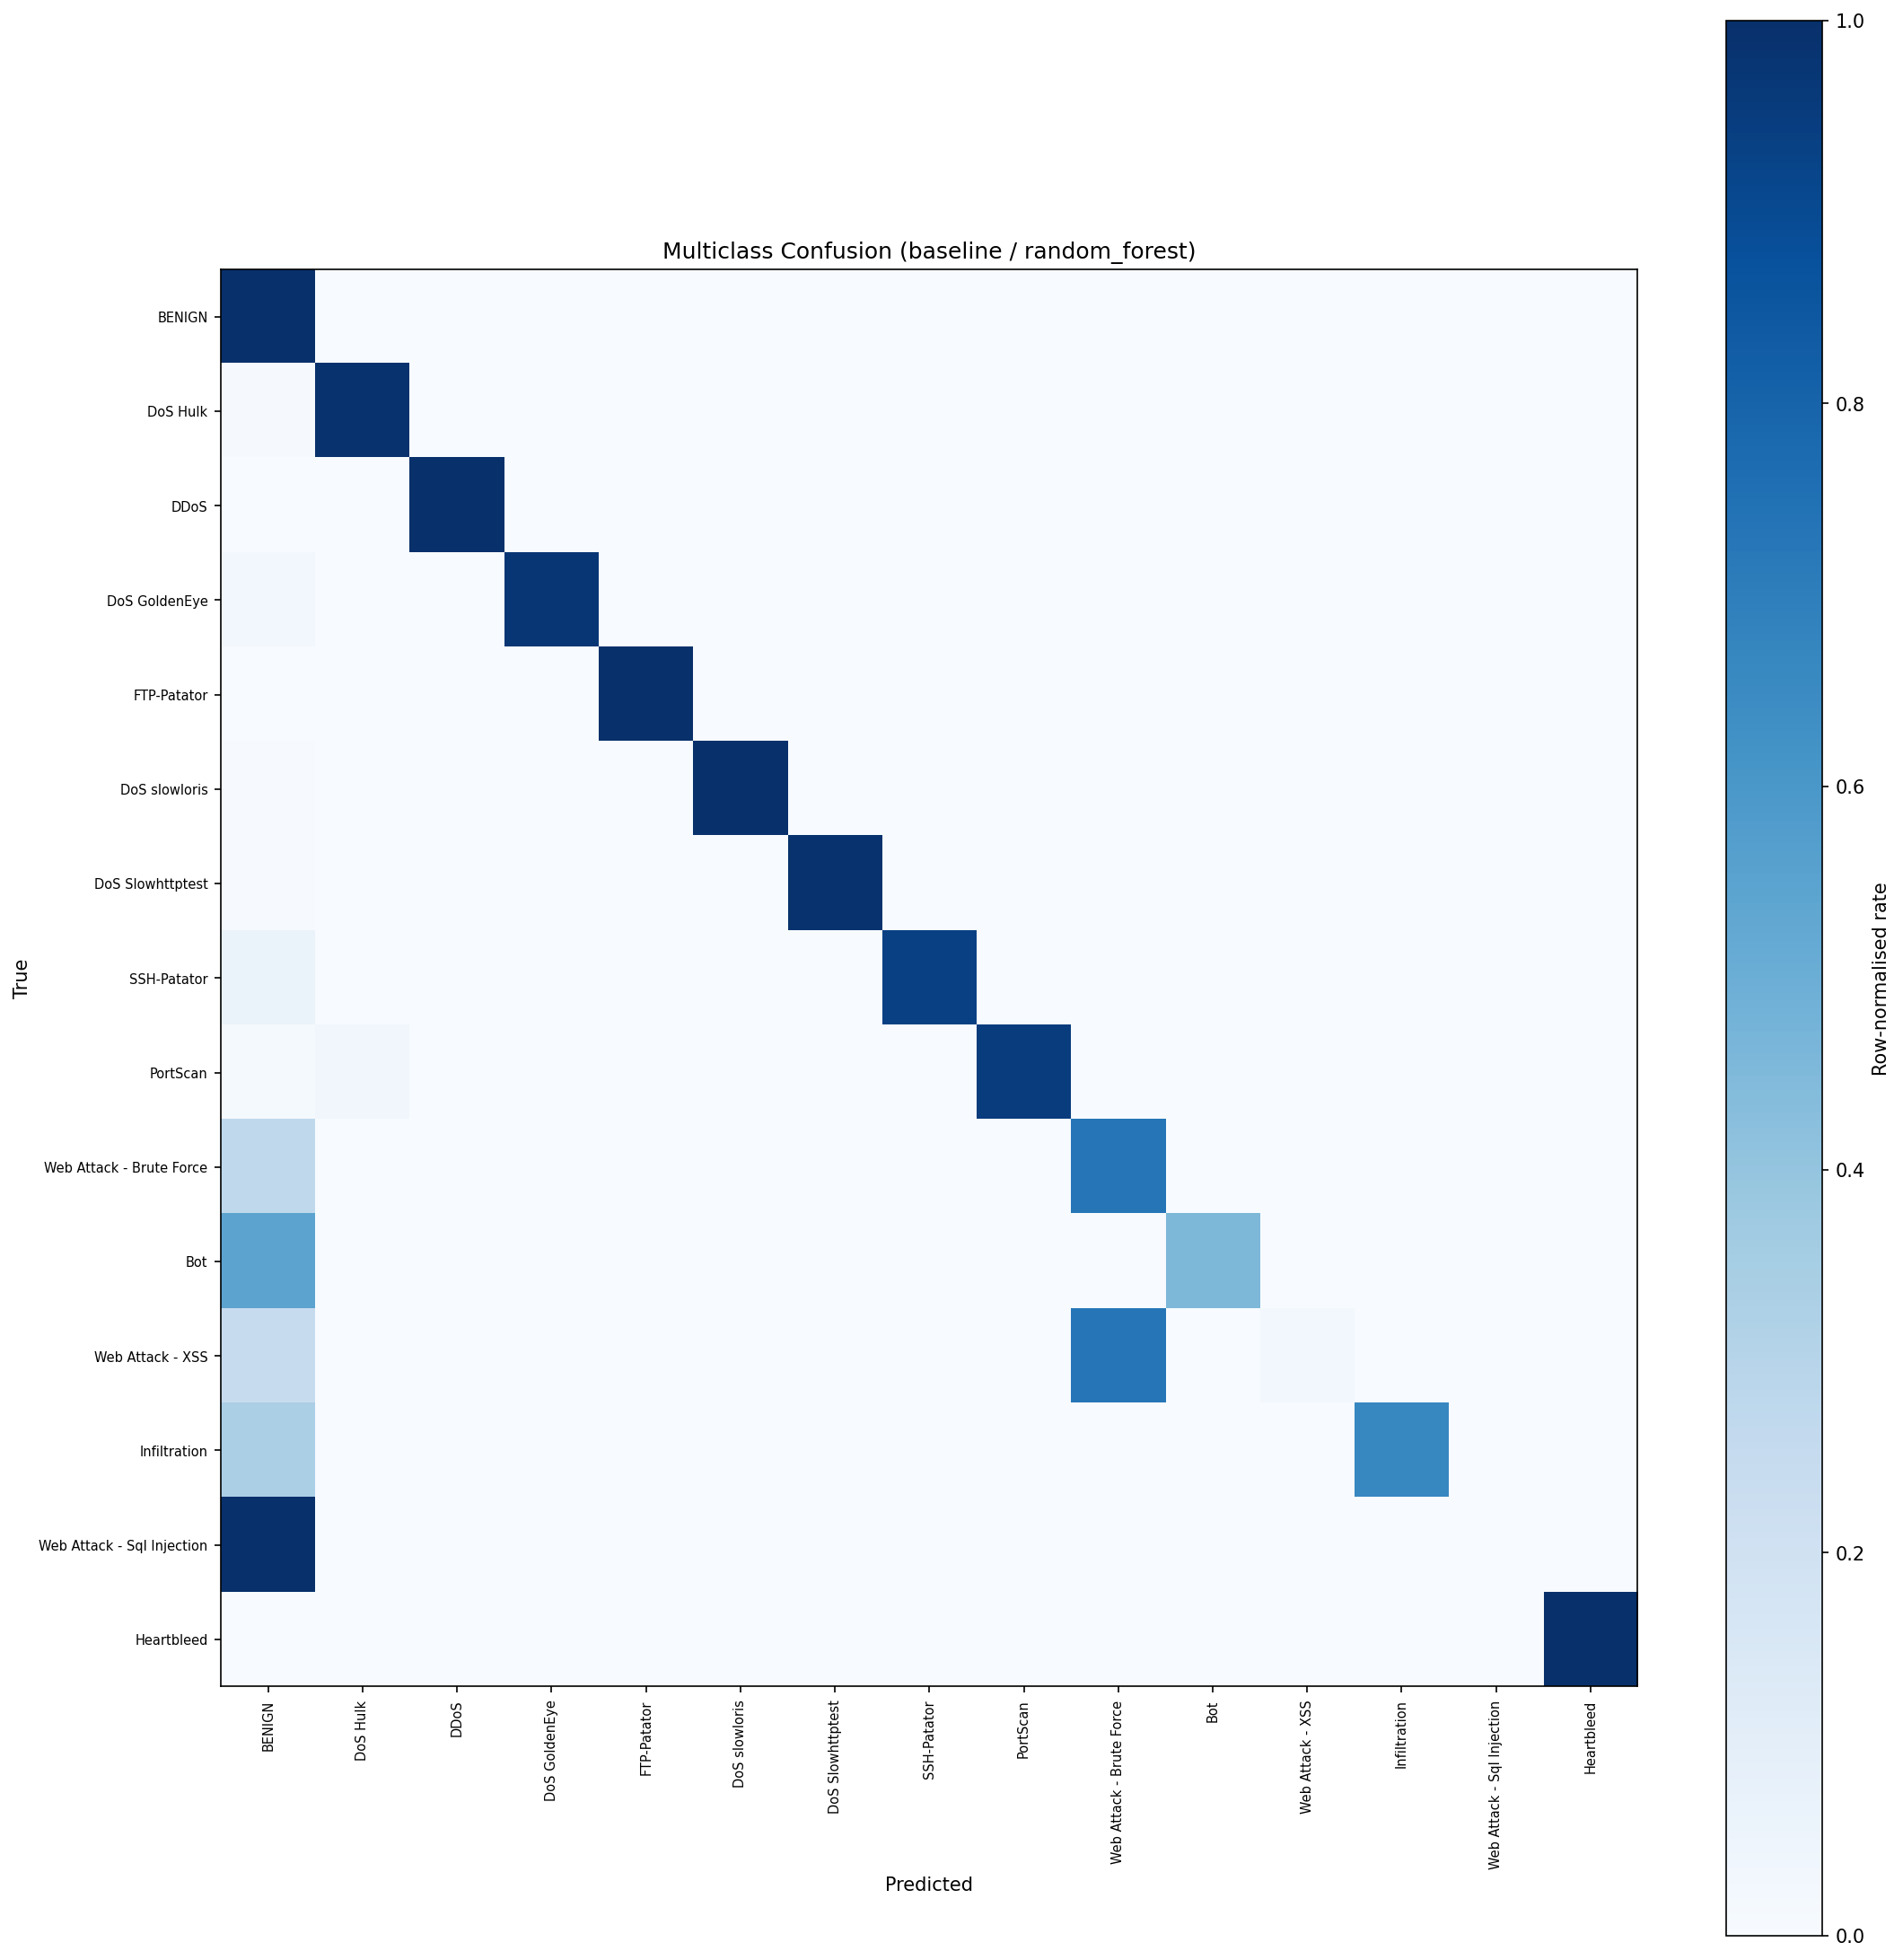
\includegraphics[width=0.7\textwidth]{img/confusion_matrix.png}}{\fbox{\parbox{0.66\textwidth}{\centering\vspace{1.4cm}\ph{Ma trận nhầm lẫn đa lớp --- chạy ml\_09\_multiclass\_eval.py}\vspace{1.4cm}}}}
    \caption{Ma trận nhầm lẫn đa lớp theo loại tấn công (chuẩn hóa theo hàng)}
    \label{fig:confusion_matrix}
\end{figure}

\textbf{Phân tích hướng nhầm lẫn giữa các lớp hiếm.} Đọc ma trận nhầm lẫn theo \emph{đích đến} của các dự đoán sai cho thấy các lớp hiếm suy giảm theo hai kiểu khác nhau. Kiểu thứ nhất là \emph{nhầm loại nhưng vẫn bị phát hiện}: 81/111 mẫu Web Attack~--~XSS bị gán thành Web Attack~--~Brute Force, tức ở bài toán nhị phân triển khai trên biên, các luồng này \emph{vẫn bị gắn cờ tấn công} (76\% XSS vẫn bị chặn), chỉ sai ở khâu định danh loại. Kiểu thứ hai nguy hiểm hơn: \emph{lọt hẳn thành Benign}: toàn bộ 6/6 mẫu SQL Injection, 158/290 mẫu Bot (54\%) và 84/311 mẫu Web Brute Force bị dự đoán là lưu lượng bình thường. Ba cơ chế giải thích hiện tượng này: (i)~\emph{mất cân bằng cực đoan} (6--311 mẫu so với 380.119 mẫu Benign) khiến các lớp hiếm gần như không có vùng quyết định riêng; (ii)~việc \emph{loại \texttt{destination\_port}} ảnh hưởng nặng nhất đến nhóm tấn công web: khi mất ``lối tắt'' cổng 80, các luồng HTTP tấn công (request/response ngắn) có đặc trưng hành vi rất gần lưu lượng duyệt web thường và gần lẫn nhau; giá trị recall 0{,}027 của XSS là con số \emph{trung thực} thay cho con số đẹp nhờ rò rỉ; (iii)~\emph{Bot lẫn Benign do bản chất}: các luồng beaconing C\&C nhỏ, đều đặn, giống lưu lượng nền khi không còn định danh cổng/dịch vụ. Nhận diện này định hướng trực tiếp cho hướng phát triển: xử lý mất cân bằng có chủ đích (tăng cường/oversampling lớp hiếm), bổ sung đặc trưng chuỗi thời gian cho hành vi beaconing, và kiểm chứng liên bộ dữ liệu (Mục~\ref{sec:cross-dataset}).

\pagebreak

\clearpage
\section{Thực nghiệm và đánh giá hiệu năng mô hình trên Jetson Orin Nano Super}

Trong phần này, luận văn đề xuất xây dựng một hệ thống phát hiện xâm nhập mạng \ac{ids} \emph{phân tán} triển khai trên một cụm \textbf{hai thiết bị biên NVIDIA Jetson Orin Nano Super}~\cite{nvidia2019jetson} nhằm đánh giá khả năng hoạt động trong môi trường tài nguyên hạn chế; đây là hướng tiếp cận điện toán biên đưa phân tích về gần nguồn dữ liệu để giảm băng thông và thời gian phản hồi \cite{shi2016edge,hamdan2020edge}, trong khi các nghiên cứu IDS biên trước đây chủ yếu đánh giá suy luận đơn nút \cite{sforzin2016rpids}. Hệ thống được thiết kế theo kiến trúc xử lý dữ liệu thời gian thực hai tầng: một \emph{cổng phát hiện bất thường} (anomaly gate) bằng autoencoder nhẹ lọc bớt lưu lượng bình thường trên Jetson~\#1, và một \emph{bộ phân loại} PySpark \texttt{PipelineModel} chỉ xử lý các luồng nghi vấn trên Jetson~\#2. Hạ tầng trung tâm (Apache Kafka cho truyền tải thông điệp, PostgreSQL để quản lý dữ liệu, InfluxDB để lưu chỉ số hiệu năng theo thời gian, Grafana để trực quan hóa và Mailtrap để kiểm thử cảnh báo qua email) chạy trên một máy chủ điều phối.

NVIDIA Jetson Orin Nano Super là một máy tính nhúng (single-board computer) tích hợp CPU kiến trúc ARM 64-bit và GPU NVIDIA, hỗ trợ tăng tốc suy luận học máy ngay tại biên; cấu hình chi tiết đã nêu tại Bảng~\ref{tab:hardware} (Chương~3) và mục Môi trường thực nghiệm. Do hạn chế về tài nguyên tính toán so với máy chủ truyền thống, việc triển khai trên Jetson Orin Nano Super cho phép đánh giá khả năng tối ưu hóa mô hình và hiệu năng suy luận trong điều kiện phần cứng nhúng (edge computing).

Mô hình có hiệu năng tối ưu được xác định ở phần đánh giá hiệu năng phân loại phía trên sẽ được tích hợp vào pipeline xử lý nhằm thực hiện nhiệm vụ phát hiện và phân loại lưu lượng mạng thành hai nhóm: \textit{Benign} và \textit{Attack}. Các chỉ số đánh giá bao gồm độ chính xác (Accuracy), Precision, Recall, F1-Score, thời gian dự đoán trung bình cho mỗi mẫu, thông lượng xử lý (throughput) và mức tiêu thụ tài nguyên hệ thống (CPU, RAM). Kết quả thực nghiệm cho phép phân tích tính khả thi của việc triển khai hệ thống \ac{ids} dựa trên học máy trong môi trường thiết bị biên có tài nguyên giới hạn.

\subsection{Các công cụ sử dụng trong hệ thống}

Trong hệ thống phát hiện xâm nhập mạng \ac{ids} được đề xuất, ngoài các công nghệ xử lý dữ liệu lớn đã trình bày ở Chương~2, luận văn sử dụng thêm một số công cụ và nền tảng mã nguồn mở nhằm hỗ trợ truyền tải dữ liệu, lưu trữ, giám sát hiệu năng và cảnh báo theo thời gian thực. Cụ thể:

\begin{itemize}

    \item \textbf{Apache Kafka}~\cite{Kreps2011} -- Là nền tảng truyền tải thông điệp phân tán (distributed event streaming platform), được sử dụng để tiếp nhận và phân phối dữ liệu luồng theo cơ chế publish-subscribe. Trong hệ thống, Kafka đóng vai trò trung gian giữa nguồn dữ liệu (CICIDS2017 được mô phỏng bằng Python script) và thiết bị Jetson Orin Nano Super, đảm bảo khả năng truyền tải bất đồng bộ, chịu lỗi và mở rộng linh hoạt.

    \item \textbf{Apache Spark Streaming} -- Là thành phần xử lý dữ liệu luồng thời gian thực. Spark Streaming nhận dữ liệu từ Kafka Consumer, thực hiện các bước tiền xử lý đặc trưng và chuyển dữ liệu đến mô hình học máy đã được huấn luyện để thực hiện suy luận.

    \item \textbf{PostgreSQL} -- Là hệ quản trị cơ sở dữ liệu quan hệ mã nguồn mở có độ ổn định và khả năng mở rộng cao. Trong hệ thống, PostgreSQL được sử dụng để lưu trữ kết quả dự đoán, thông tin cảnh báo và các bản ghi phục vụ báo cáo tổng hợp.

    \item \textbf{InfluxDB} -- Là cơ sở dữ liệu chuỗi thời gian (Time-Series Database), tối ưu cho việc lưu trữ và truy vấn các chỉ số theo thời gian. Hệ thống sử dụng InfluxDB để ghi nhận các thông số hiệu năng như thời gian suy luận, mức sử dụng CPU, bộ nhớ và thông lượng xử lý.

    \item \textbf{Grafana} -- Là nền tảng trực quan hóa dữ liệu mã nguồn mở, cho phép xây dựng các dashboard theo thời gian thực. Grafana kết nối với InfluxDB và PostgreSQL để hiển thị tình trạng hoạt động của hệ thống \ac{ids} cũng như thống kê các sự kiện tấn công.

    \item \textbf{Mailtrap} -- Là công cụ kiểm thử email trong môi trường giả lập. Trong giai đoạn thực nghiệm, Mailtrap được sử dụng để kiểm tra cơ chế gửi cảnh báo khi hệ thống phát hiện lưu lượng mạng bất thường trước khi triển khai môi trường thực tế.

\end{itemize}

Việc tích hợp các công nghệ trên giúp hệ thống đảm bảo khả năng xử lý dữ liệu thời gian thực, lưu trữ an toàn, giám sát hiệu năng liên tục và kích hoạt cảnh báo kịp thời khi phát hiện hành vi xâm nhập.

\pagebreak
\subsection{Mô hình hệ thống đề xuất}
Hệ thống phát hiện xâm nhập được thiết kế theo kiến trúc xử lý dữ liệu luồng như minh họa ở Hình~\ref{fig:ids_diagram}. Luồng xử lý tổng thể bao gồm các bước sau:
\begin{figure}[ht]
    \centering
    \resizebox{\textwidth}{!}{%
    \begin{tikzpicture}[
        font=\small, >=Stealth,
        every node/.style={align=center},
        pc/.style ={draw=gray!60,         thick, rounded corners, fill=gray!8,  minimum width=13.4cm, minimum height=1.3cm, inner sep=3pt},
        jet/.style={draw=accGreen!80!black,  thick, rounded corners, fill=accGreen!8, text width=4.2cm, minimum height=2.0cm, inner sep=4pt},
        mtr/.style={draw=accBlue,         thick, rounded corners, fill=accBlue!5,  minimum width=13.4cm, minimum height=1.0cm, inner sep=3pt},
        lbl/.style={font=\footnotesize, fill=white, inner sep=1.5pt, align=center, text=accBlue!75!black},
        arr/.style ={-{Stealth[length=2.5mm]}, thick, draw=gray!60!black},
        dsh/.style={-{Stealth[length=2.5mm]}, thick, draw=accBlue, dashed},
    ]
        \node[pc]  (pc)  at (0, 0.0)   {\textbf{Máy chủ điều phối (MacBook, Docker)}\\[2pt]
            Apache Kafka \;$|$\; PostgreSQL \;$|$\; InfluxDB \;$|$\; Grafana \;$|$\; \texttt{data\_sender.py}};
        \node[jet] (j1)  at (-4.6,-4.7) {\textbf{Jetson Orin Nano Super \#1}\\[2pt] \texttt{anomaly\_gate}\\[2pt]
            Autoencoder lọc bớt\\ lưu lượng bình thường};
        \node[jet] (j2)  at ( 4.6,-4.7) {\textbf{Jetson Orin Nano Super \#2}\\[2pt] \texttt{classifier}\\[2pt]
            PySpark \texttt{PipelineModel}\\ phân loại Benign / Attack};
        \node[mtr] (out) at (0,-9.0)    {Chỉ số hiệu năng $\rightarrow$ InfluxDB $\rightarrow$ Grafana \quad$|$\quad
            Cảnh báo: Email (Mailtrap) / Slack};

        \draw[arr] (pc.south -| j1) -- node[lbl]{topic\\ \texttt{ids-network-flow}} (j1.north);
        \draw[arr] (j1.east) -- node[lbl]{\texttt{ids-suspicious-flow}\\ (luồng nghi vấn)} (j2.west);
        \draw[arr] (j2.north) -- node[lbl]{kết quả phân loại\\ $\rightarrow$ PostgreSQL} (pc.south -| j2);
        % Mũi tên gạch đứt (metric/cảnh báo) đi thẳng vào CẠNH TRÊN của dải, không cắt chữ.
        \draw[dsh] (j1.south) -- (out.north -| j1);
        \draw[dsh] (j2.south) -- (out.north -| j2);
    \end{tikzpicture}%
    }
    \caption[Kiến trúc hệ thống IDS phân tán trên cụm 2 Jetson Orin Nano Super]{Kiến trúc hệ thống phát hiện xâm nhập phân tán thời gian thực trên cụm 2 Jetson Orin Nano Super}
    \label{fig:ids_diagram}
\end{figure}

\pagebreak
\begin{enumerate}

    \item \textbf{Nguồn dữ liệu}:
    Dữ liệu từ bộ CICIDS2017 được mô phỏng theo thời gian thực thông qua một Python script và gửi vào Kafka Producer trên topic \texttt{ids-network-flow}.

    \item \textbf{Cổng phát hiện bất thường (Jetson~\#1)}:
    Jetson~\#1 đảm nhận vai trò \texttt{anomaly\_gate}: một autoencoder nhẹ (huấn luyện chỉ trên lưu lượng bình thường) tính sai số tái tạo (reconstruction error) cho từng luồng. Các luồng có sai số dưới ngưỡng được coi là bình thường và \emph{được lọc bỏ}; chỉ các luồng \emph{nghi vấn} mới được chuyển tiếp sang topic \texttt{ids-suspicious-flow}. Cơ chế này giảm đáng kể khối lượng phải đưa vào suy luận Spark.

    \item \textbf{Bộ phân loại (Jetson~\#2)}:
    Jetson~\#2 đảm nhận vai trò \texttt{classifier}: tải mô hình PySpark \texttt{PipelineModel} (với tập đặc trưng SHAP Top-30 đã chọn) và phân loại các luồng nghi vấn thành \textit{Benign} hoặc \textit{Attack}. Vector đầu vào khi triển khai gồm 29 đặc trưng: trong Top-30 theo xếp hạng SHAP có \texttt{destination\_port}, nhưng đặc trưng này bị loại khỏi mô hình xuất ra để triển khai vì là kênh rò rỉ nhãn trên CICIDS2017 (Mục~\ref{sec:leakage_analysis}), nhất quán với giao thức chống rò rỉ ở pha huấn luyện.

    \item \textbf{Ghi nhận hiệu năng}:
    Mỗi nút ghi nhận thời gian dự đoán/mẫu, mức sử dụng CPU/RAM/nhiệt độ và thông lượng (gắn nhãn theo \texttt{EDGE\_NODE\_ID}); các chỉ số được lưu vào InfluxDB.

    \item \textbf{Lưu trữ và cảnh báo}:
    Kết quả dự đoán và sự kiện tấn công được lưu vào PostgreSQL; khi phát hiện lưu lượng bất thường, hệ thống kích hoạt cảnh báo qua Email/\allowbreak Webhook (Mailtrap, Slack trong môi trường kiểm thử) từ một nút chính được chỉ định để tránh trùng lặp.

    \item \textbf{Trực quan hóa và giám sát}:
    Grafana truy xuất dữ liệu từ InfluxDB và PostgreSQL để xây dựng dashboard theo thời gian thực, giám sát trạng thái hệ thống và thống kê các sự kiện tấn công.

\end{enumerate}

\textbf{Ba chế độ triển khai phân tán.} Cụm hai Jetson hỗ trợ ba chế độ, lựa chọn theo ràng buộc tải và độ trễ:
\begin{itemize}
    \item \textbf{Chế độ A -- Pipeline split} (khuyến nghị): Jetson~\#1 = cổng bất thường (anomaly gate), Jetson~\#2 = bộ phân loại (classifier) (như mô tả trên), giúp giảm tải Spark nhờ lọc lưu lượng bình thường sớm.
    \item \textbf{Chế độ B -- Mở rộng theo chiều ngang (Horizontal scaling)}: cả hai Jetson chạy pipeline đầy đủ trong cùng một nhóm tiêu thụ (consumer group) của Kafka nhằm tăng thông lượng.
    \item \textbf{Chế độ C -- Spark cluster}: máy chủ MacBook làm Spark master, hai Jetson làm worker, phân tán suy luận Spark trên cụm. Nhất quán với nguyên tắc ở mục Môi trường thực nghiệm, MacBook chỉ đảm nhận điều phối (master), không chạy executor; toàn bộ tính toán suy luận vẫn nằm trên hai Jetson.
\end{itemize}

Kiến trúc này đảm bảo tính mô-đun, tách biệt các thành phần xử lý, đồng thời phù hợp với mô hình triển khai phân tán trên các thiết bị biên có tài nguyên hạn chế như Jetson Orin Nano Super.

\textbf{Đặc tả cổng bất thường (operating point).} Cổng autoencoder là một bộ lọc \emph{điều chỉnh được} chứ không phải một điểm cố định: nâng ngưỡng giúp giảm tải (offload) nhiều lưu lượng bình thường hơn khỏi Spark (tăng tỷ lệ bỏ qua tại cổng, gate-skip) nhưng có thể giảm recall trên lớp tấn công. Ngưỡng của cổng được chọn theo phân vị (quantile) của sai số tái tạo tính trên một \emph{tập kiểm định benign}, gồm 10\% tách từ phần lưu lượng bình thường của tập huấn luyện (\texttt{seed}=42); tập kiểm tra không tham gia việc chọn ngưỡng, tránh rò rỉ kiểu ``ngưỡng oracle''. Bảng~\ref{tab:gate_oc} trình bày đường đánh đổi giữa recall và mức giảm tải (recall--offload) khi quét các mức quantile trên tập kiểm định này; điểm vận hành được chọn theo ngân sách độ trễ/độ chính xác của triển khai. FPR trong bảng là tỷ lệ luồng benign bị cổng chuyển nhầm sang bộ phân loại, không phải FPR của toàn hệ thống.

\begin{table}[htbp]
\centering
\caption[Điểm vận hành của cổng bất thường theo ngưỡng quantile]{Điểm vận hành của cổng bất thường theo ngưỡng quantile trên tập kiểm định benign}
\label{tab:gate_oc}
\begin{tabular*}{\textwidth}{@{\extracolsep{\fill}}ccccc@{}}
\toprule
\textbf{Quantile (validation)} & \textbf{Ngưỡng} & \textbf{Recall (Attack)} & \textbf{FPR} & \textbf{Tỷ lệ bỏ qua tại cổng (\%)} \\ \midrule
0{,}90 & 0{,}0023 & 0{,}7589 & 0{,}1003 & 80{,}08 \\
0{,}95 & 0{,}0052 & 0{,}7552 & 0{,}0506 & 84{,}36 \\
0{,}99 & 0{,}0192 & 0{,}7420 & 0{,}0101 & 88{,}00 \\
0{,}995 & 0{,}0317 & 0{,}7229 & 0{,}0053 & 88{,}70 \\ \bottomrule
\end{tabular*}
\end{table}


\subsection{Lựa chọn mô hình cho thiết bị biên}

Triển khai trên thiết bị biên đặt ra các ràng buộc về tài nguyên: RAM 8\,GB chia sẻ giữa CPU và GPU (trong đó PySpark JVM chiếm một phần đáng kể), CPU ARM, cùng ràng buộc về nhiệt độ/băng thông tại biên. Cũng cần nhấn mạnh rằng việc chọn Apache Spark trên Jetson 8\,GB phải chịu chi phí JVM/Spark đáng kể; Spark được dùng ở đây nhằm \emph{nhất quán} với pha huấn luyện phân tán, chứ không nhằm tối ưu độ trễ suy luận trên một nút; chi phí đánh đổi này được định lượng qua so sánh với scikit-learn và ONNX Runtime ở mục~\ref{sec:engine-baseline-thesis}, còn tăng tốc bằng TensorRT là hướng nghiên cứu tương lai. Ba mô hình đại diện cho ba thử nghiệm khác nhau được chọn để đánh giá:

\begin{enumerate}
    \item \textbf{Decision Tree} -- Mô hình cây đơn lẻ, đại diện cho cách tiếp cận đơn giản nhất.
    \item \textbf{\ac{gbt} (Gradient-Boosted Trees)} -- Đại diện cho phương pháp Boosting, sử dụng nhiều cây yếu kết hợp tuần tự.
    \item \textbf{Random Forest} -- Đại diện cho phương pháp Bagging, sử dụng ensemble 200 cây song song.
\end{enumerate}

Cả ba mô hình đều được huấn luyện trên tập SHAP Top-30 đặc trưng và triển khai dưới dạng PySpark PipelineModel.

% LƯU Ý: terminal + Grafana đã chụp lại từ cụm Jetson (2026-07-19). Riêng 2 ảnh
% cảnh báo email/Slack dùng lại ảnh giai đoạn thử nghiệm sớm — chính văn dưới cụm
% hình đã ghi chú tường minh; mô-đun cảnh báo không đổi giữa hai giai đoạn.
\begin{figure}[htbp]
    \centering
    \IfFileExists{img/pipeline_terminal_jetson1.png}{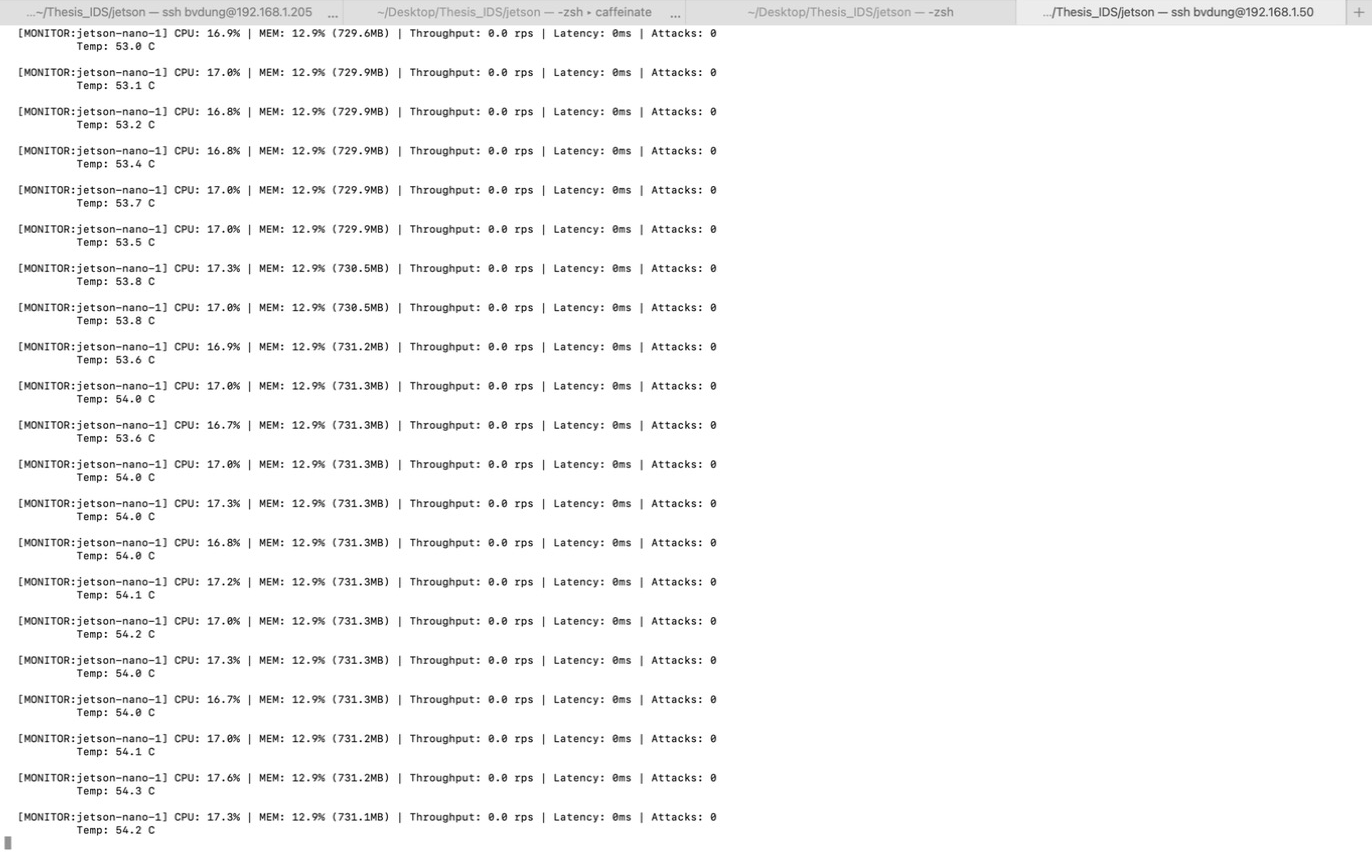
\includegraphics[width=0.85\textwidth]{img/pipeline_terminal_jetson1.png}}{\fbox{\parbox{0.85\textwidth}{\centering\vspace{1.2cm}\ph{Ảnh terminal node cổng (jetson-nano-1)}\vspace{1.2cm}}}}\\[2pt]
    {\footnotesize (a) Jetson \#1 (\texttt{jetson-nano-1}): cổng phát hiện bất thường, giám sát tài nguyên theo node}\\[8pt]
    \IfFileExists{img/pipeline_terminal_jetson2.png}{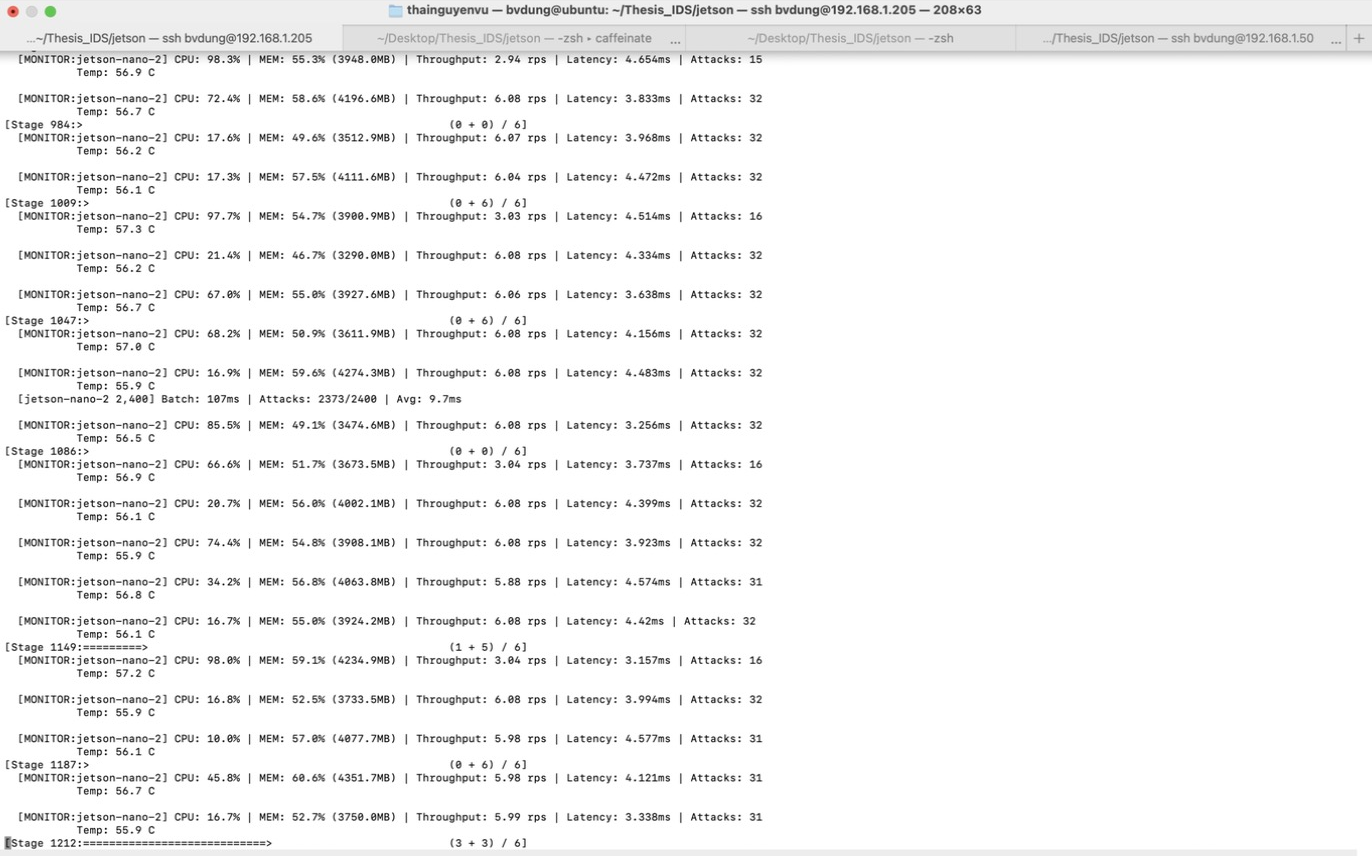
\includegraphics[width=0.85\textwidth]{img/pipeline_terminal_jetson2.png}}{\fbox{\parbox{0.85\textwidth}{\centering\vspace{1.2cm}\ph{Ảnh terminal node phân loại (jetson-nano-2)}\vspace{1.2cm}}}}\\[2pt]
    {\footnotesize (b) Jetson \#2 (\texttt{jetson-nano-2}): bộ phân loại PySpark, thông lượng \textasciitilde6 luồng/giây, độ trễ suy luận \textasciitilde4\,ms, đếm tấn công theo lô}
    \caption[Giao diện terminal của pipeline IDS trên hai node Jetson]{Giao diện terminal của pipeline IDS trên hai node Jetson: (a) cổng lọc bất thường, (b) bộ phân loại PySpark}
    \label{fig:pipeline_terminal}
\end{figure}

\begin{figure}[htbp]
    \centering
    \IfFileExists{img/grafana_dashboard.png}{
\includegraphics[width=0.9\textwidth]{img/grafana_dashboard.png}}{\fbox{\parbox{0.85\textwidth}{\centering\vspace{1.2cm}\ph{Dashboard Grafana hiệu năng --- chụp lại từ cụm Jetson}\vspace{1.2cm}}}}
    \caption{Dashboard Grafana giám sát hiệu năng IDS theo thời gian thực}
    \label{fig:grafana_dashboard}
\end{figure}


\begin{figure}[htbp]
    \centering
    \IfFileExists{img/mailtrap_alert.png}{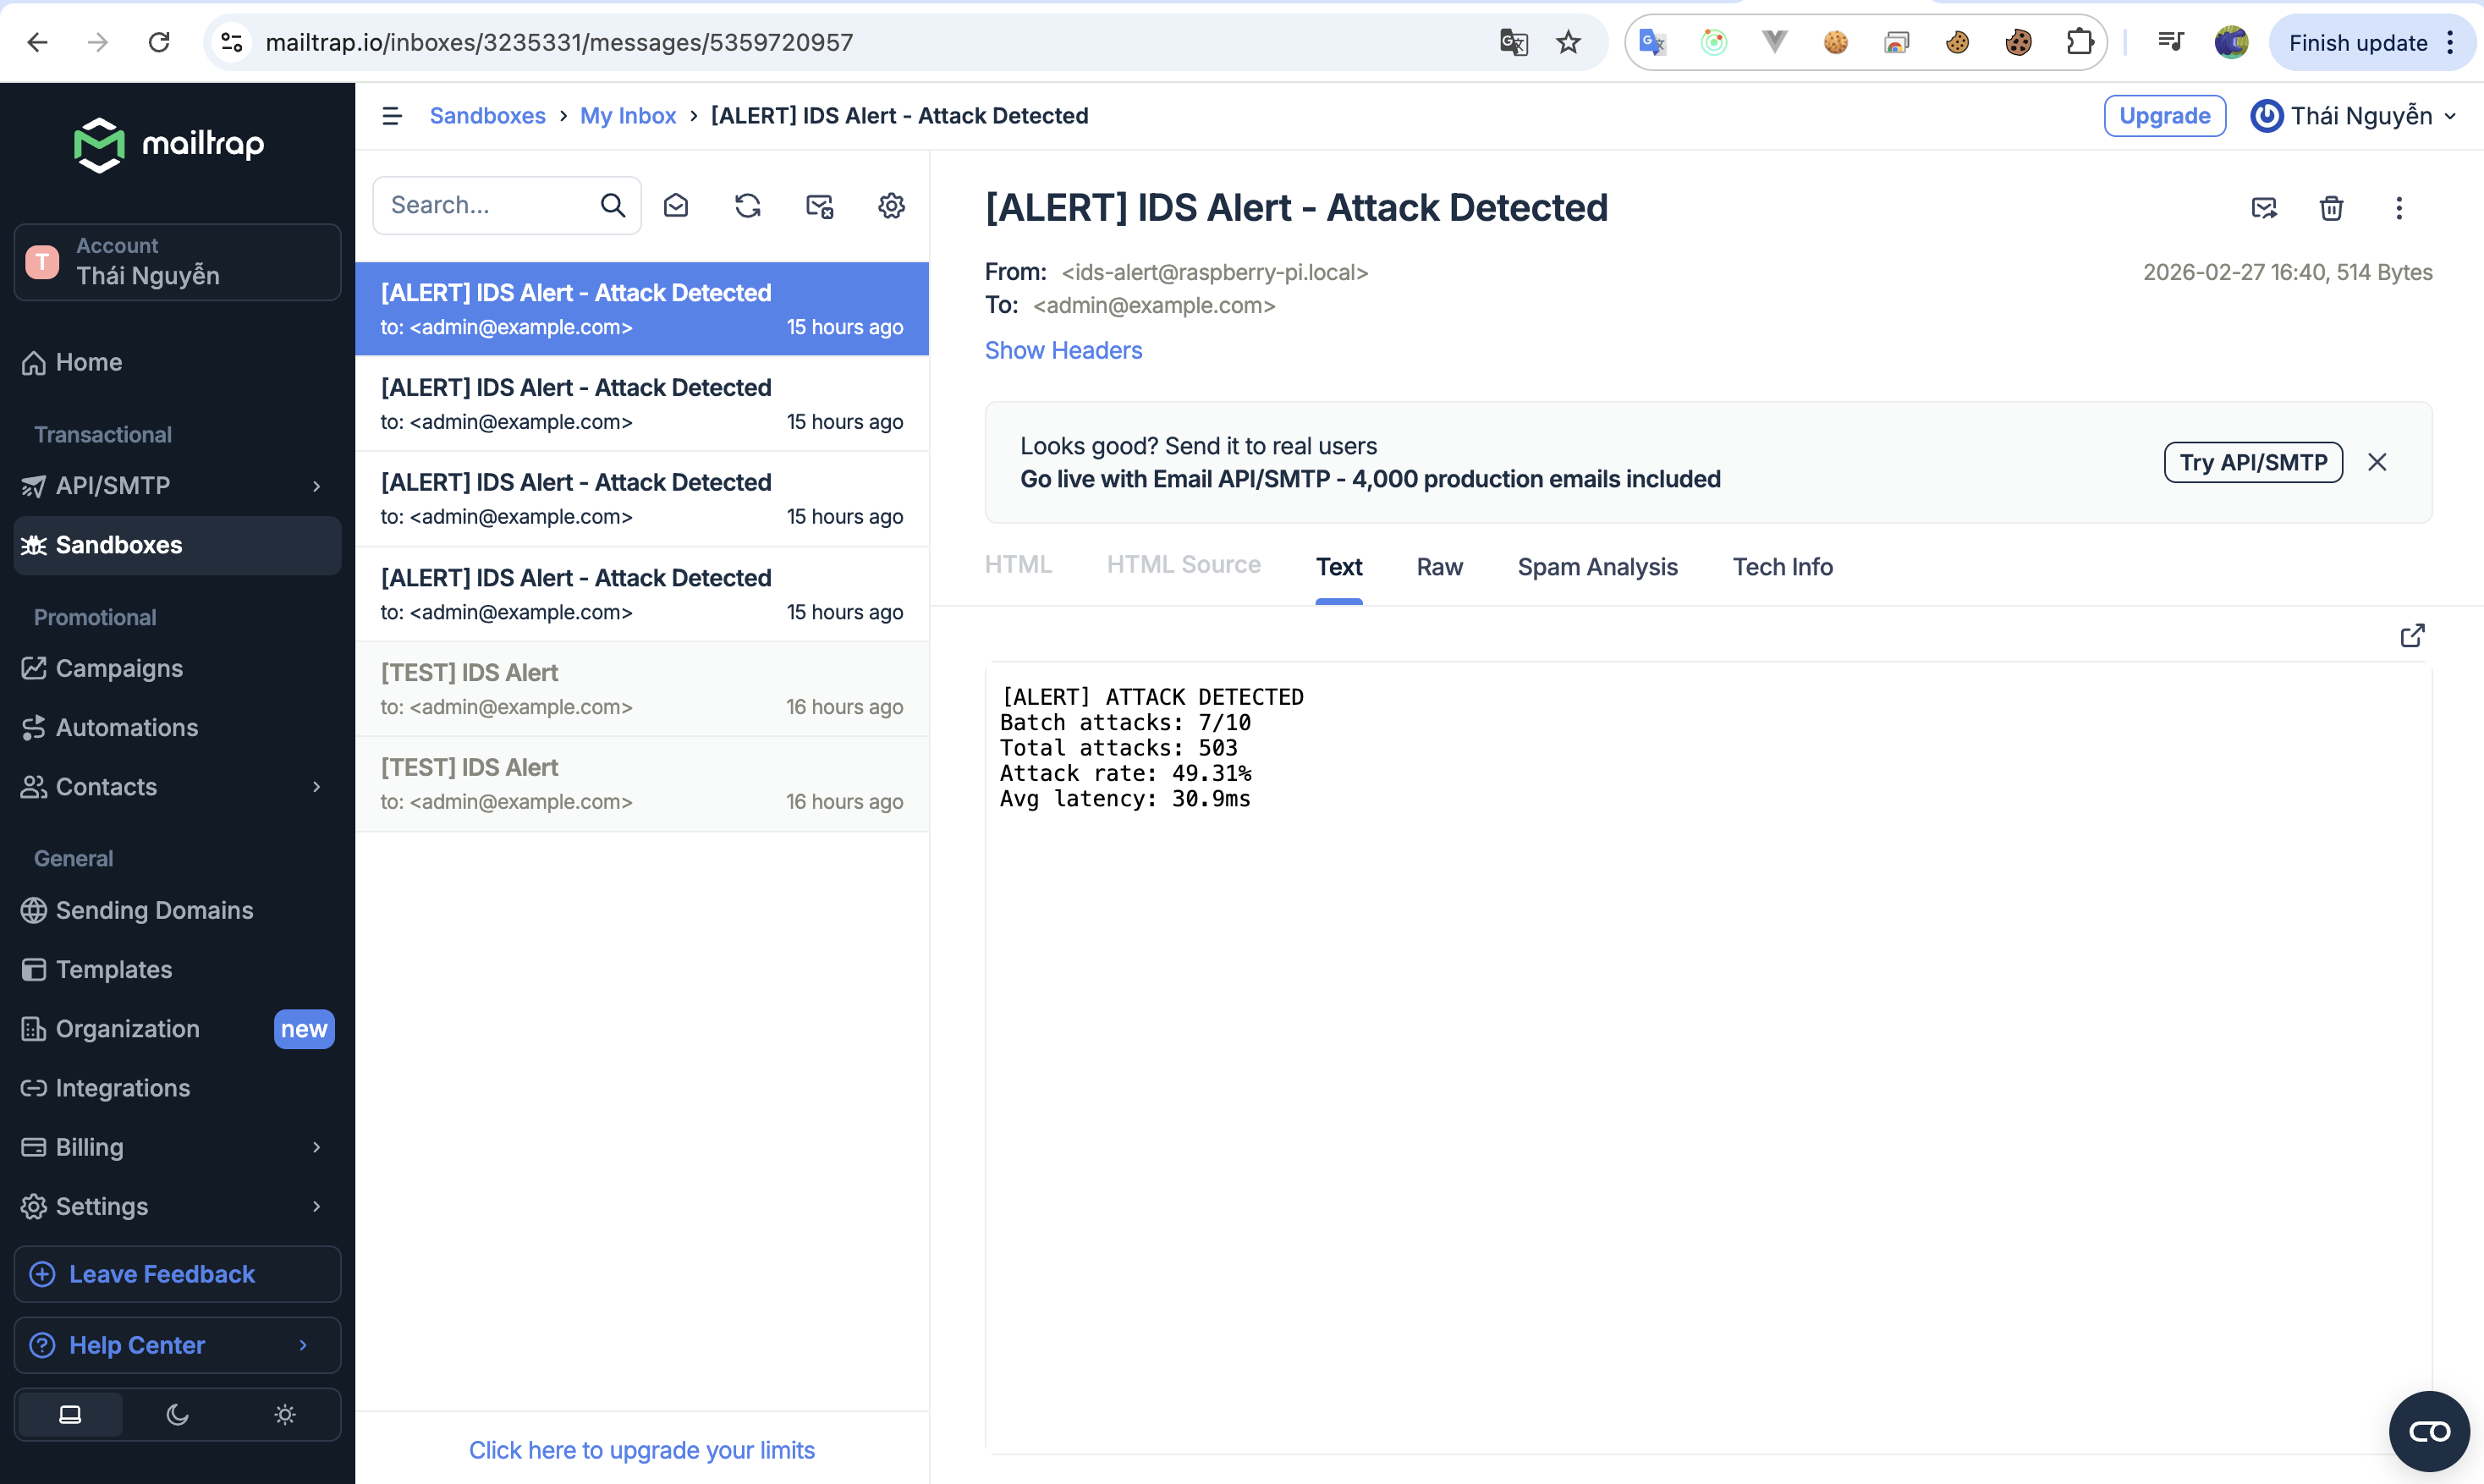
\includegraphics[width=0.9\textwidth]{img/mailtrap_alert.png}}{\fbox{\parbox{0.85\textwidth}{\centering\vspace{1.2cm}\ph{Email cảnh báo Mailtrap --- chụp lại từ hệ chạy trên Jetson}\vspace{1.2cm}}}}
    \caption[Email cảnh báo tấn công gửi qua Mailtrap]{Email cảnh báo tấn công gửi qua Mailtrap trong môi trường kiểm thử}
    \label{fig:mailtrap_alert}
\end{figure}

\begin{figure}[htbp]
    \centering
    \IfFileExists{img/grafana_attacks.png}{
\includegraphics[width=0.9\textwidth]{img/grafana_attacks.png}}{\fbox{\parbox{0.85\textwidth}{\centering\vspace{1.2cm}\ph{Dashboard Grafana chi tiết tấn công --- chụp lại từ cụm Jetson}\vspace{1.2cm}}}}
    \caption[Dashboard Grafana chi tiết các cuộc tấn công được phát hiện]{Dashboard Grafana hiển thị chi tiết các cuộc tấn công được phát hiện và phân loại theo thời gian}
    \label{fig:grafana_attacks}
\end{figure}

\begin{figure}[htbp]
    \centering
    \IfFileExists{img/grafana_peak_load.png}{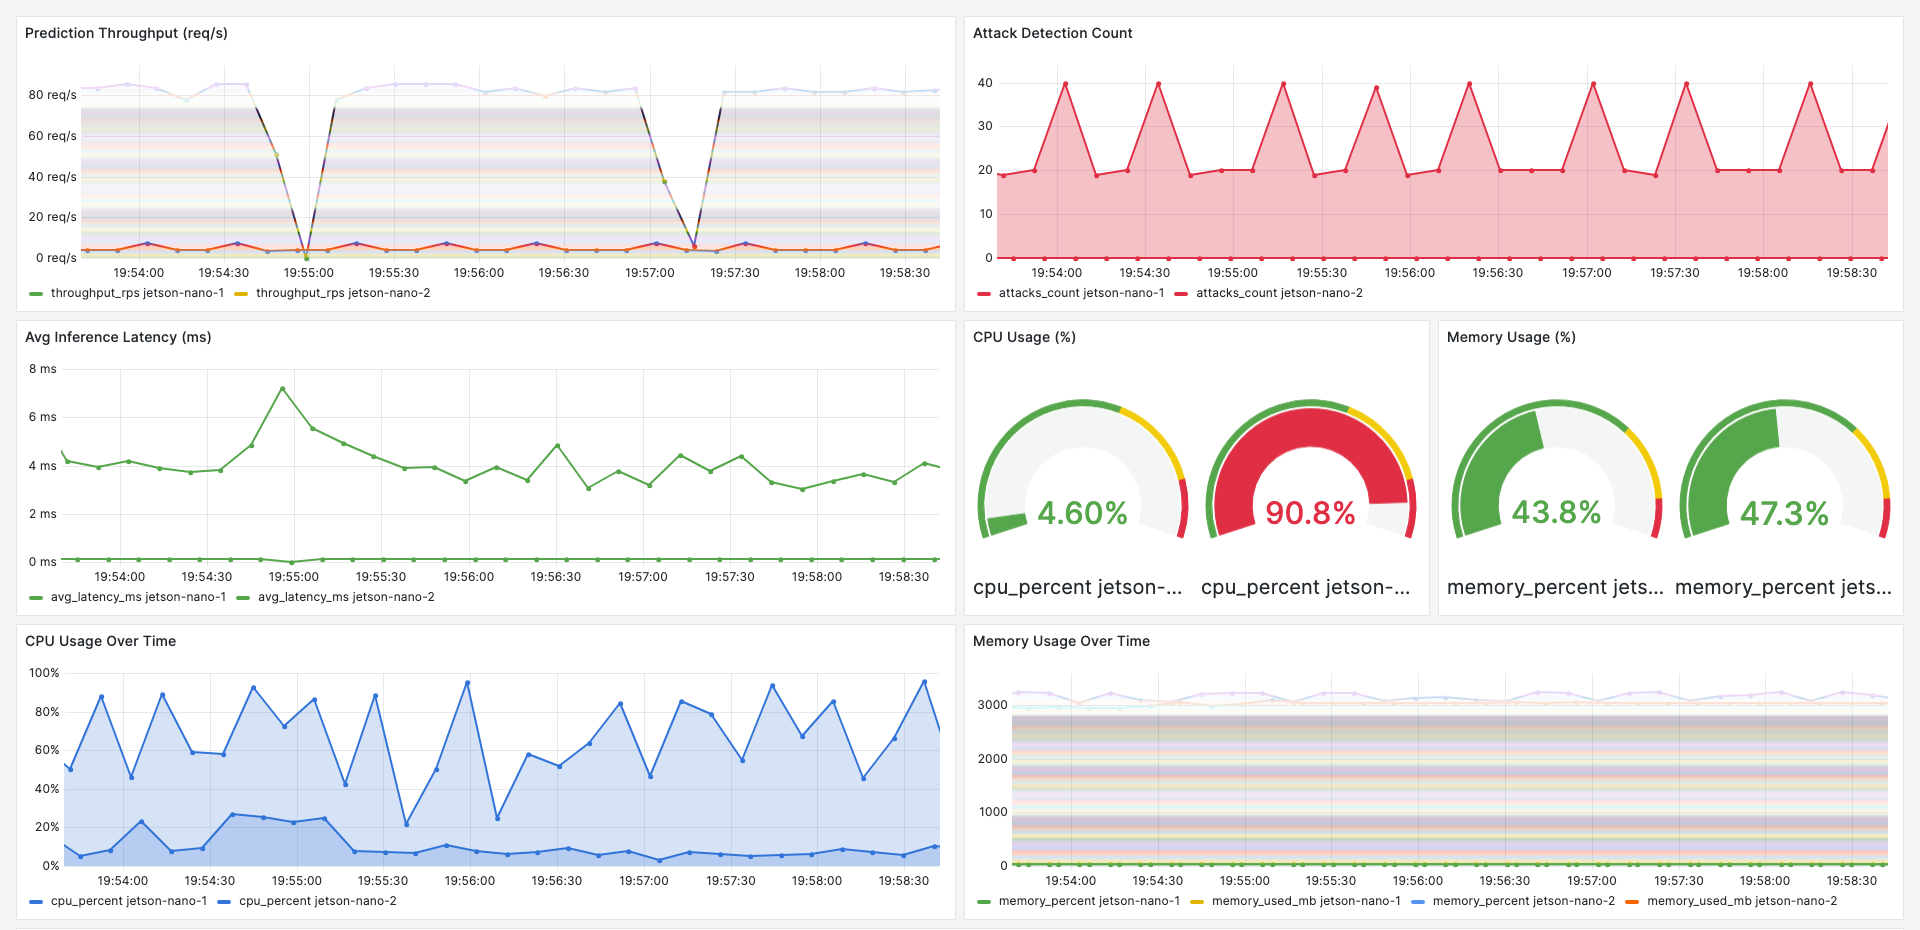
\includegraphics[width=0.9\textwidth]{img/grafana_peak_load.png}}{\fbox{\parbox{0.85\textwidth}{\centering\vspace{1.2cm}\ph{Dashboard Grafana tại thời điểm tải đỉnh --- chụp lại từ cụm Jetson}\vspace{1.2cm}}}}
    \caption[Dashboard Grafana tại thời điểm tải đỉnh của chế độ tách pipeline]{Dashboard Grafana tại thời điểm tải đỉnh của chế độ tách pipeline}
    \label{fig:grafana_peak_load}
\end{figure}

\begin{figure}[htbp]
    \centering
    \IfFileExists{img/slack_alert.png}{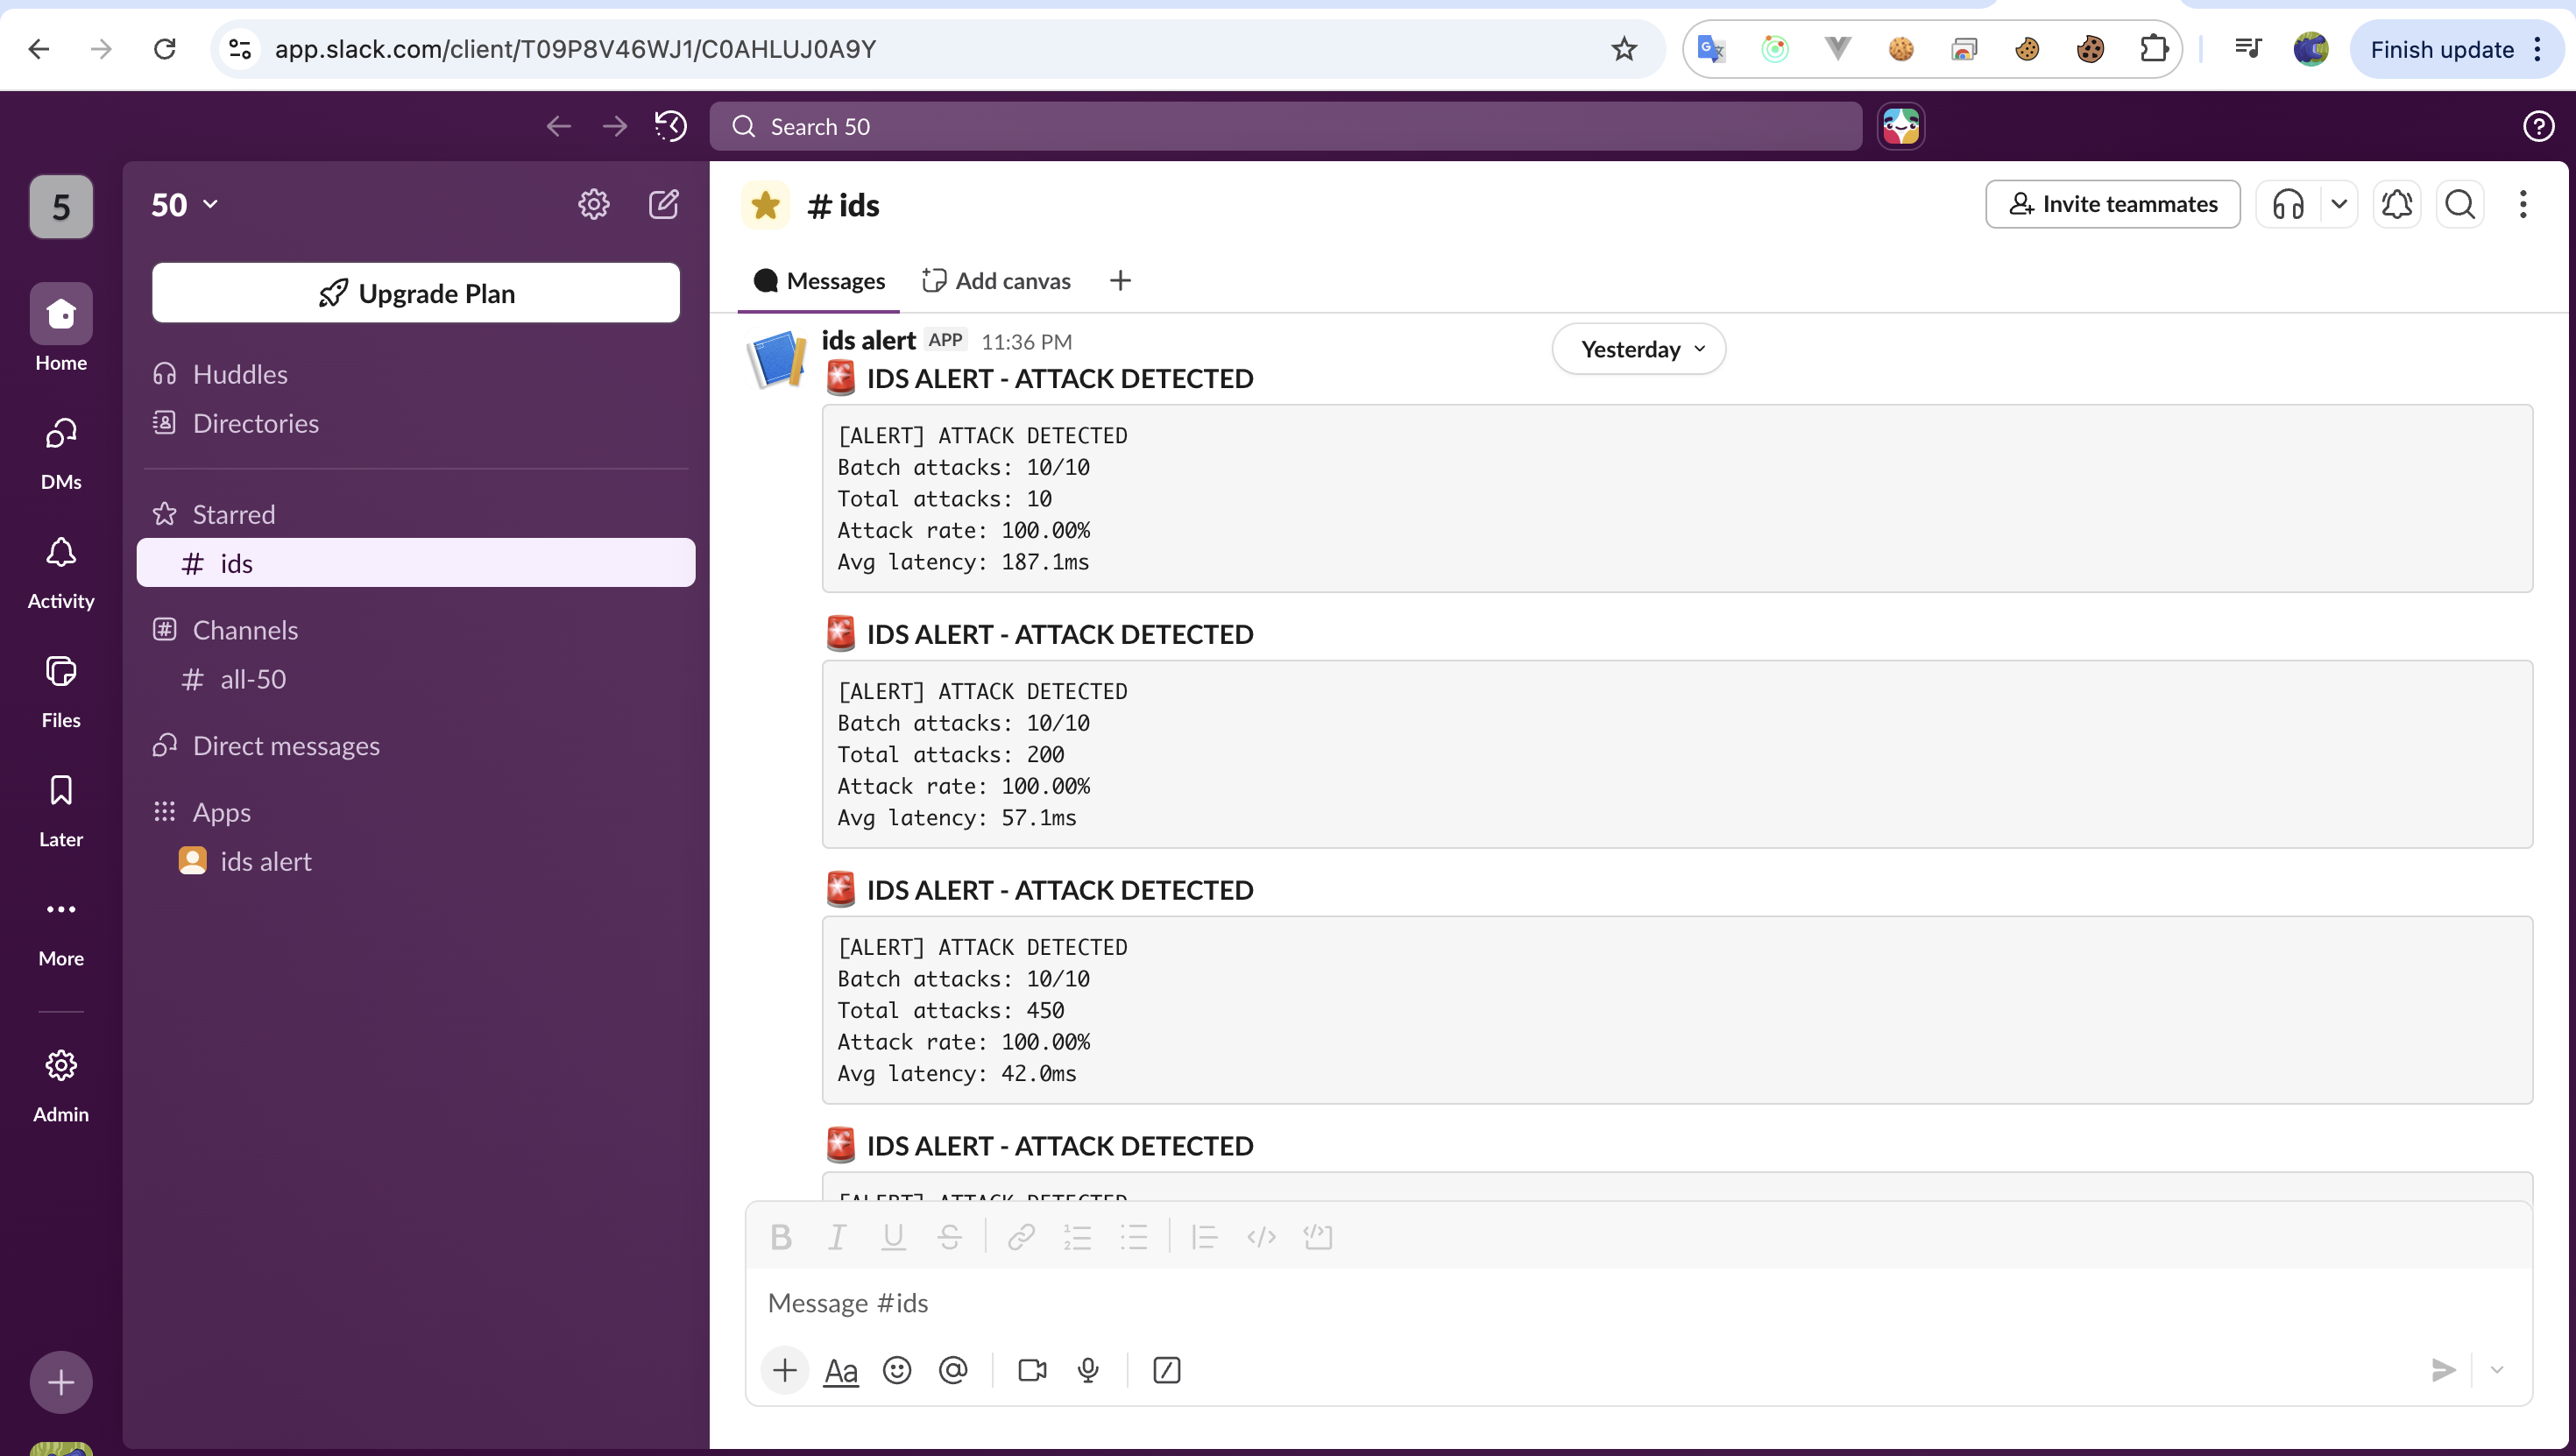
\includegraphics[width=0.9\textwidth]{img/slack_alert.png}}{\fbox{\parbox{0.85\textwidth}{\centering\vspace{1.2cm}\ph{Thông báo Slack --- chụp lại từ hệ chạy trên Jetson}\vspace{1.2cm}}}}
    \caption[Thông báo cảnh báo tấn công gửi qua Slack]{Thông báo cảnh báo tấn công gửi qua Slack Incoming Webhook}
    \label{fig:slack_alert}
\end{figure}

Hình~\ref{fig:pipeline_terminal} minh họa giao diện terminal thực tế khi pipeline IDS đang xử lý dữ liệu trên Jetson Orin Nano Super, bao gồm thông tin về thông lượng, độ trễ và số lượng tấn công phát hiện được. Hai dashboard Grafana (Hình~\ref{fig:grafana_dashboard} và Hình~\ref{fig:grafana_attacks}) cho phép giám sát hiệu năng hệ thống và chi tiết các cuộc tấn công theo thời gian thực. Hình~\ref{fig:grafana_peak_load} ghi lại thời điểm tải đỉnh, cho thấy rõ sự phân bố tải lệch đặc trưng của chế độ tách pipeline: nút cổng chỉ sử dụng khoảng 5\,\% CPU trong khi nút phân loại PySpark đạt tới 91\,\%, xác nhận bộ phân loại là thành phần chiếm tài nguyên chủ đạo và là căn cứ cho các phân tích năng lượng--thông lượng ở phần sau. Khi phát hiện tấn công, hệ thống tự động gửi cảnh báo qua nhiều kênh: email thông qua Mailtrap SMTP (Hình~\ref{fig:mailtrap_alert}) và tin nhắn Slack (Hình~\ref{fig:slack_alert}). Hai ảnh cảnh báo này chụp từ giai đoạn thử nghiệm sớm của hệ thống; mô-đun cảnh báo và định dạng thông điệp giữ nguyên khi triển khai trên cụm Jetson.
\subsection{Kết quả huấn luyện các mô hình ứng viên trên cụm Spark}

Bảng \ref{tab:edge_training} trình bày kết quả huấn luyện và đánh giá ba mô hình ứng viên trên cụm Spark (mô tả ở mục Môi trường thực nghiệm) trước khi triển khai xuống thiết bị biên.

\begin{table}[htbp]
\centering
\caption[Các mô hình ứng viên cho triển khai biên (SHAP Top-30)]{Kết quả huấn luyện các mô hình ứng viên cho triển khai biên (SHAP Top-30)}
\label{tab:edge_training}
\begin{tabular*}{\textwidth}{@{\extracolsep{\fill}}lcccc@{}}
\toprule
\textbf{Mô hình} & \textbf{F1-Score} & \textbf{Accuracy} & \textbf{Thời gian huấn luyện (s)} & \textbf{Kích thước (MB)} \\ \midrule
Decision Tree    & 0{,}9814 & 0{,}9943 & 24{,}4  & 0{,}046 \\
\ac{gbt}              & 0{,}9753 & 0{,}9925 & 341{,}8 & 0{,}865 \\
Random Forest    & 0{,}9826 & 0{,}9947 & 687{,}3 & 4{,}427 \\
\bottomrule
\end{tabular*}
\end{table}

Về tiêu chí \emph{nhận biết ràng buộc biên} (edge-aware), ba mô hình ứng viên đánh đổi khác nhau: Decision Tree có kích thước nhỏ nhất (0,046\,MB, nhỏ hơn Random Forest khoảng 96 lần) và huấn luyện nhanh hơn khoảng 28 lần, trong khi Random Forest đạt F1 cao nhất. Riêng F1/Accuracy chưa đủ để kết luận: quyết định cuối cùng dựa trên số đo vận hành thực tế trên thiết bị (thông lượng, độ trễ, CPU, RAM) ở mục tiếp theo. (Các mô hình ứng viên biên được huấn luyện trên mẫu con phân tầng khi xuất để vừa bộ nhớ một nút, nên F1 thấp hơn chút ít so với kết quả huấn luyện phân tán đầy đủ ở Bảng~\ref{tab:summary_comparison}; độ chính xác chính thức lấy từ pha huấn luyện đầy đủ.)


\subsection{Kết quả đo hiệu năng (benchmark) trên Jetson Orin Nano Super}

Bảng \ref{tab:edge_benchmark} trình bày kết quả đo hiệu năng (benchmark) thực tế trên Jetson Orin Nano Super. Mỗi cấu hình được đo lặp lại 5 lần; trước mỗi cửa sổ đo có giai đoạn khởi động (warm-up) bằng chính lưu lượng thật để làm nóng JVM/JIT, và dữ liệu warm-up bị loại khỏi cửa sổ đo; kết quả báo cáo là trung bình $\pm$ độ lệch chuẩn qua các lần chạy. Hai loại độ trễ được ghi nhận: (i) \emph{độ trễ suy luận} (tiền xử lý + dự đoán) trên từng nút, và (ii) \emph{độ trễ đầu cuối} (từ thời điểm producer gửi đến khi có phán quyết) tính từ nhãn thời gian của producer; giá trị tuyệt đối của loại (ii) chỉ có ý nghĩa khi các máy đồng bộ đồng hồ NTP. Các phân vị độ trễ (p50/p95/p99) được tính ở mức từng lần chạy từ \emph{log thô theo từng luồng} trong đúng cửa sổ tải; với cụm nhiều nút, p95 báo cáo là p95 của nút xấu nhất (không lấy phân vị của các giá trị trung bình theo nút).

\begin{table}[htbp]
\centering
\caption{So sánh hiệu năng triển khai trên Jetson Orin Nano Super}
\label{tab:edge_benchmark}
\small
\begin{tabular*}{\textwidth}{@{\extracolsep{\fill}}lccccc@{}}
\toprule
\textbf{Mô hình} & \textbf{Thông lượng} & \textbf{Độ trễ suy luận (ms)} & \textbf{CPU} & \textbf{RAM} & \textbf{Kích thước} \\
                  & \textbf{(mẫu/giây)} & \textbf{p50 / p95 / p99} & \textbf{(\%)} & \textbf{(\%)} & \textbf{(MB)} \\ \midrule
Decision Tree     & 22{,}0 & 441 / 537 / -- & 46{,}4 & 21{,}9 & 0{,}046 \\
\ac{gbt}               & 24{,}3 & 414 / 439 / -- & 40{,}9 & 24{,}0 & 0{,}865 \\
Random Forest     & 26{,}8 & 378 / 397 / -- & 35{,}2 & 27{,}5 & 4{,}427 \\
\bottomrule
\end{tabular*}
\end{table}

\subsection{So sánh engine suy luận: chi phí của việc đồng nhất stack}
\label{sec:engine-baseline-thesis}
Luận văn triển khai mô hình dưới dạng \texttt{PipelineModel} của Spark để \emph{đồng nhất với pha huấn luyện phân tán}: cùng một stack vừa huấn luyện trên cụm vừa suy luận trên thiết bị. Để \emph{định lượng chi phí đánh đổi} của sự đồng nhất này, luận văn đo lại \emph{cùng một} mô hình Random Forest (cùng siêu tham số) trên \emph{cùng} tập đặc trưng SHAP đã chọn để triển khai nhưng qua các engine nhẹ hơn ở chế độ một nút: scikit-learn (CPU, không JVM) và ONNX Runtime (CPU execution provider; Bảng~\ref{tab:engines_thesis}, sinh từ \texttt{benchmark\_engines.py}). Cả ba engine được đo trên nút phân loại với batch 10; năng lượng báo cáo là phần \emph{hoạt động}, đã trừ nền idle. Vì cùng thuật toán và đặc trưng nên độ chính xác tương đương; phép so sánh tập trung vào \emph{chi phí suy luận}. (Cả ba dòng của Bảng~\ref{tab:engines_thesis} được đo lại trong \emph{cùng một phiên} trên cùng trạng thái bo mạch để so sánh công bằng, nên dòng PySpark chênh lệch nhỏ so với Bảng~\ref{tab:edge_benchmark} đo ở phiên trước: 22,6 so với 26,8 luồng/giây, do khác phiên đo và xung CPU.) Kết quả đo (Bảng~\ref{tab:engines_thesis}) cho thấy stack JVM/Spark chịu chi phí suy luận cao hơn đáng kể so với scikit-learn trên bo mạch ARM 8\,GB: thông lượng thấp hơn khoảng 9 lần, độ trễ p95 cao hơn khoảng 11 lần, tỷ lệ RAM gần gấp đôi và năng lượng mỗi suy luận cao hơn khoảng 25 lần. Biên dịch cùng mô hình rừng ngẫu nhiên sang ONNX Runtime còn nới rộng khoảng cách này đáng kể: $\approx$7\,900 luồng/giây với p95 1,1\,ms, tức gấp $\approx$348 lần thông lượng của Spark đã triển khai, ở mức năng lượng chỉ $\approx$2\% so với scikit-learn; việc nêu rõ điều này là cơ sở cho hướng phát triển \emph{xuất mô hình sang ONNX/TensorRT để suy luận} trong khi vẫn giữ Spark cho huấn luyện (việc tích hợp phiên ONNX vào pipeline streaming và khai thác GPU qua TensorRT thuộc hướng phát triển).

\begin{table}[htbp]
\centering
\caption[Chi phí suy luận một nút: Spark, sklearn và ONNX]{Chi phí suy luận một nút trên cùng mô hình và tập đặc trưng: Spark, sklearn và ONNX}
\label{tab:engines_thesis}
\renewcommand{\arraystretch}{1.1}
\small
\begin{tabular*}{\textwidth}{@{\extracolsep{\fill}}lcccc@{}}
\toprule
\textbf{Engine} & \textbf{\shortstack{Thông lượng\\(luồng/giây)}} & \textbf{\shortstack{Độ trễ\\p95 (ms)}} & \textbf{RAM (\%)} & \textbf{\shortstack{Năng lượng\\/suy luận (mJ)}} \\ \midrule
PySpark (triển khai) & 22{,}6 & 532 & 24{,}3 & 71{,}6 \\
scikit-learn         & 204{,}4 & 49{,}8 & 13{,}3 & 2{,}91 \\
ONNX Runtime         & 7870{,}8 & 1{,}1 & 15{,}7 & 0{,}06 \\
\bottomrule
\end{tabular*}
\end{table}

\subsection{Kết quả ba chế độ triển khai phân tán}

Ngoài việc so sánh các mô hình trên một nút, luận văn đánh giá ba chế độ triển khai phân tán trên cụm hai Jetson Orin Nano Super (Bảng~\ref{tab:edge_modes}). Chỉ số chính gồm thông lượng, độ trễ p95 (ms), tỷ lệ bỏ qua tại cổng (gate-skip: \% lưu lượng bình thường được cổng lọc khỏi suy luận Spark) và F1 trên lớp tấn công. \emph{Thông lượng} được định nghĩa là số \emph{phán quyết cuối cùng} ghi vào PostgreSQL trên giây (một luồng nhận phán quyết hoặc tại cổng (nếu bị bỏ qua là benign) hoặc tại bộ phân loại), không cộng dồn đầu ra của hai tầng để tránh đếm trùng luồng được chuyển tiếp ở chế độ pipeline split.

\begin{table}[htbp]
\centering
\caption{So sánh ba chế độ triển khai phân tán trên cụm 2 Jetson Orin Nano Super}
\label{tab:edge_modes}
\small
\begin{tabular*}{\textwidth}{@{\extracolsep{\fill}}lccccc@{}}
\toprule
\textbf{Chế độ} & \textbf{\shortstack{Thông lượng\\(luồng/giây)}} & \textbf{\shortstack{Độ trễ\\p95 (ms)}} & \textbf{\shortstack{Bỏ qua\\tại cổng (\%)}} & \textbf{\shortstack{Năng lượng\\/suy luận (mJ)}} & \textbf{\shortstack{F1\\(Attack)}} \\ \midrule
Một nút (single)        & 2{,}60 $\pm$ 0{,}41 & 12{,}3 $\pm$ 3{,}0 & (nội tuyến) & 2490 & $\dagger$ \\
A: Pipeline split       & 62{,}5 $\pm$ 0{,}6  & 13{,}1 $\pm$ 2{,}6 & 95{,}8      & 178  & $\dagger$ \\
B: Horizontal scaling   & 5{,}9 $\pm$ 1{,}4   & 21{,}6 $\pm$ 19{,}2 & (nội tuyến) & 2250 & $\dagger$ \\
C: Spark cluster        & 90{,}0 $\pm$ 25{,}6 & 23{,}9 $\pm$ 17{,}8 & 97{,}9      & 119  & $\dagger$ \\ \bottomrule
\end{tabular*}

\tabnote{Phát lại CICIDS2017 ở 100 luồng/giây; trung bình $\pm$ độ lệch chuẩn trên $\geq$3 lần lặp; p95 tính từ log thô từng luồng (nút xấu nhất). ``(nội tuyến)'': ở vai trò \texttt{full}, cổng chạy trong cùng tiến trình và các luồng bị bỏ qua vẫn được ghi phán quyết nên không có tỷ lệ bỏ qua riêng. $\dagger$: chất lượng phát hiện không phụ thuộc chế độ (các chế độ dùng cùng một mô hình xuất ra); F1 lớp tấn công ngoại tuyến xem Bảng~\ref{tab:leakage_ablation}.}
\end{table}

\begin{figure}[htbp]
    \centering
    \IfFileExists{img/edge_modes.png}{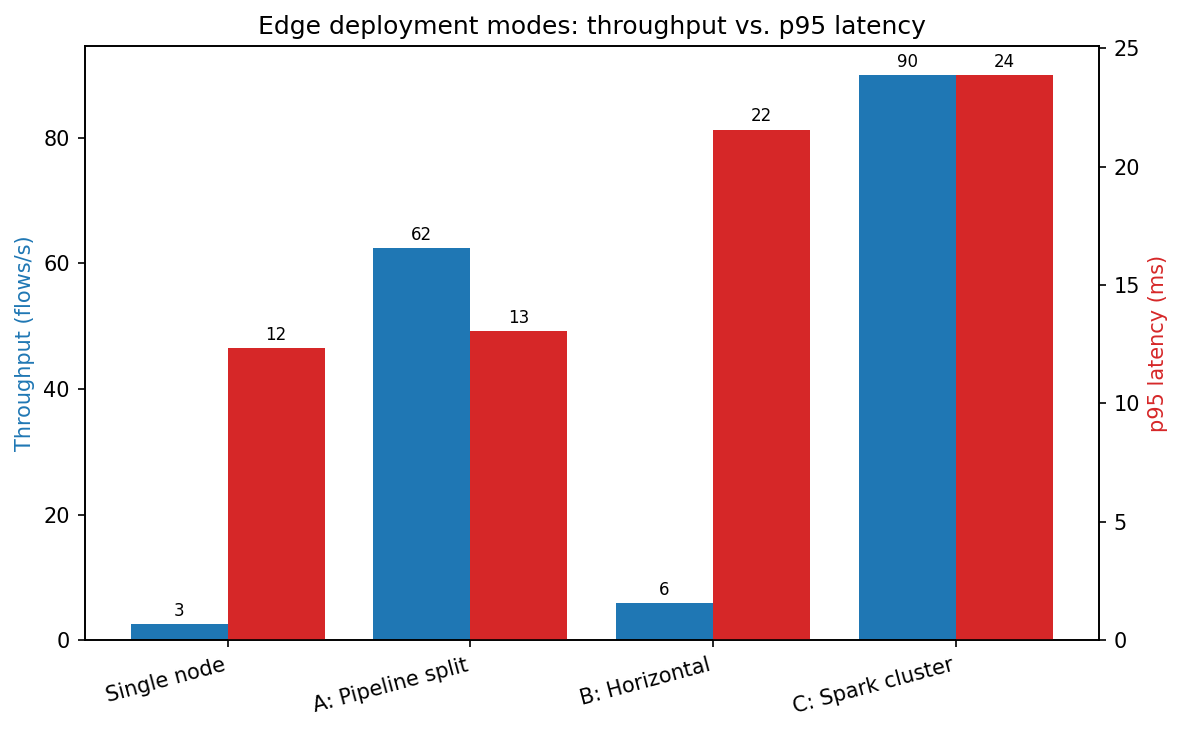
\includegraphics[width=0.95\textwidth]{img/edge_modes.png}}{\fbox{\parbox{0.8\textwidth}{\centering\vspace{1.2cm}\ph{Biểu đồ so sánh chế độ triển khai --- chạy plot\_edge\_modes.py}\vspace{1.2cm}}}}
    \caption[Thông lượng và độ trễ p95 của bốn cấu hình triển khai]{Thông lượng và độ trễ p95 của bốn cấu hình (một nút cơ sở + ba chế độ phân tán) trên cụm 2 Jetson}
    \label{fig:edge_modes}
\end{figure}

Kết quả thực đo (Hình~\ref{fig:edge_modes}) cho thấy: chế độ \emph{pipeline split} tách cổng khỏi bộ phân loại Spark giúp thông lượng phán quyết tăng từ 2{,}6 lên 62{,}5 luồng/giây (gấp $\approx$24 lần) với p95 gần như không đổi, nhờ cổng lọc 95{,}8\% lưu lượng bình thường và không còn bị Spark chặn vòng xử lý. \emph{Mở rộng theo chiều ngang} chỉ tăng xấp xỉ gấp đôi một nút (5{,}9 so với 2{,}6) vì mỗi nút vẫn chạy trọn bộ phân loại Spark trong tiến trình. \emph{Spark cluster} (cổng + bộ phân loại nối cụm Spark standalone) đạt thông lượng trung bình cao nhất (90{,}0) nhưng dao động lớn giữa các lần chạy ($\pm$26) và phụ thuộc thêm nút chủ (master) trên máy điều phối, nên pipeline split vẫn là khuyến nghị mặc định. \emph{Năng lượng mỗi suy luận} đo bằng \texttt{tegrastats} (nền idle 30\,giây trước mỗi cửa sổ tải; chế độ hai nút cộng công suất cả hai bo mạch): ở mức tải 100 luồng/giây, phần công suất \emph{hoạt động} (đã trừ idle) nằm dưới ngưỡng nhiễu lấy mẫu ($<$0{,}15\,W mọi nút), do đó bảng báo cáo năng lượng \emph{toàn bo mạch} trên mỗi phán quyết, tức thước đo mức dàn trải công suất bo mạch theo thông lượng ở cấp triển khai (không phải chi phí riêng của mô hình): các chế độ dùng cổng (A, C) dàn trải công suất hai bo mạch trên số phán quyết lớn gấp 24--35 lần, giảm năng lượng mỗi phán quyết từ $\approx$2{,}5\,J xuống 0{,}12--0{,}18\,J.

\pagebreak

\subsection{Phân tích và lựa chọn mô hình}

Hình~\ref{fig:benchmark_comparison} minh họa trực quan sự khác biệt giữa ba mô hình về thông lượng, độ trễ và mức sử dụng RAM trên Jetson Orin Nano Super.

\begin{figure}[htbp]
    \centering
    \IfFileExists{img/benchmark_comparison.png}{
\includegraphics[width=0.85\textwidth]{img/benchmark_comparison.png}}{\fbox{\parbox{0.8\textwidth}{\centering\vspace{1.4cm}\ph{Biểu đồ so sánh hiệu năng --- tạo từ \texttt{benchmark\_comparison.json}}\vspace{1.4cm}}}}
    \caption{So sánh hiệu năng ba mô hình trên Jetson Orin Nano Super}
    \label{fig:benchmark_comparison}
\end{figure}

Kết quả benchmark cho thấy sự đánh đổi rõ ràng giữa các chỉ số:

\begin{itemize}
    \item \textbf{Random Forest} thắng ở cả ba chỉ số vận hành quan trọng nhất với phát hiện xâm nhập thời gian thực: thông lượng cao nhất (26{,}8 mẫu/giây), độ trễ p95 thấp nhất (397\,ms) và CPU thấp nhất (35{,}2\%), nhờ Spark song song hóa tốt trên nhiều cây. Cái giá phải trả là RAM cao nhất (27{,}5\%) và mô hình lớn nhất ($\approx$4{,}4\,MB).
    \item \textbf{\ac{gbt}} có hiệu năng trung bình ở tất cả các chỉ số, đóng vai trò cầu nối giữa Decision Tree và Random Forest.
    \item \textbf{Decision Tree} nhẹ nhất về bộ nhớ (RAM 21{,}9\%, mô hình $\approx$0{,}05\,MB) nhưng chậm nhất: thông lượng 22{,}0 mẫu/giây và độ trễ p95 537\,ms, cao hơn Random Forest khoảng 35\%.
\end{itemize}

Hình~\ref{fig:model_tradeoff} thể hiện sự đánh đổi đa chiều giữa các tiêu chí lựa chọn mô hình: Decision Tree chiếm ưu thế về bộ nhớ, còn Random Forest chiếm ưu thế về tốc độ xử lý và tải CPU.

\begin{figure}[htbp]
    \centering
    \IfFileExists{img/model_tradeoff_radar.png}{
\includegraphics[width=0.75\textwidth]{img/model_tradeoff_radar.png}}{\fbox{\parbox{0.7\textwidth}{\centering\vspace{1.4cm}\ph{Biểu đồ radar trade-off --- tạo từ \texttt{benchmark\_comparison.json}}\vspace{1.4cm}}}}
    \caption[Biểu đồ radar đánh đổi giữa các mô hình trên thiết bị biên]{Biểu đồ radar thể hiện sự đánh đổi (trade-off) giữa các mô hình trên thiết bị biên}
    \label{fig:model_tradeoff}
\end{figure}

\textbf{Random Forest được chọn} làm mô hình triển khai chính trên thiết bị biên dựa trên ba tiêu chí:
\begin{enumerate}
    \item \textbf{Hiệu năng xử lý thời gian thực}: thông lượng cao nhất (26{,}8 mẫu/giây) và độ trễ p95 thấp nhất (397\,ms). Với \ac{ids}, độ trễ phán quyết là ràng buộc trực tiếp --- một mô hình nhỏ nhưng chậm hơn 35\% về p95 sẽ kéo dài cửa sổ mà tấn công chưa bị chặn.
    \item \textbf{Chất lượng phát hiện}: cao nhất trong ba mô hình ứng viên ở \emph{cả hai} phép đo --- F1 0{,}9955 trên đánh giá ngoại tuyến đầy đủ (Bảng~\ref{tab:summary_comparison}) và 0{,}9826 ở bản xuất huấn luyện trên mẫu con để vừa bộ nhớ một nút (Bảng~\ref{tab:edge_training}).
    \item \textbf{Tương thích nền tảng}: Random Forest là estimator gốc của Spark ML nên \texttt{PipelineModel} xuất ra nạp được trực tiếp trên bo mạch ARM64, không cần các thư viện native mà tích hợp \ac{xgb} của Spark đòi hỏi.
\end{enumerate}

Đánh đổi được chấp nhận là mức tiêu thụ bộ nhớ: Random Forest dùng 27{,}5\% RAM so với 21{,}9\% của Decision Tree và mô hình nặng $\approx$4{,}4\,MB so với 0{,}05\,MB. Trên bo mạch 8\,GB, khoảng chênh này còn dư địa lớn, nên bộ nhớ không phải là ràng buộc quyết định; Decision Tree vẫn là phương án dự phòng hợp lý nếu triển khai xuống các thiết bị \ac{iot} eo hẹp bộ nhớ hơn.

\section{Thảo luận và So sánh tổng hợp}
Kết quả thực nghiệm cho thấy lựa chọn đặc trưng dựa trên \ac{shap} là hướng tiếp cận phù hợp cho hệ thống \ac{ids} trên bộ dữ liệu CICIDS2017: dưới cấu hình đánh giá loại trừ rò rỉ dữ liệu, \ac{shap} Top-30 giữ được hiệu năng gần như nguyên vẹn trong khi cắt khoảng 60\% số đặc trưng. Ngược lại, học tổ hợp \emph{không} mang lại lợi thế trên chính cấu hình này: Hybrid Bagging đạt F1 0{,}9966 và Soft Voting đạt 0{,}9967, đều \emph{thấp hơn} \ac{xgb} đơn lẻ (0{,}9970). Học tổ hợp chỉ vượt mô hình đơn ở những cấu hình mà mô hình đơn yếu hơn (\ac{rf} Top-30: 0{,}9938 so với 0{,}9922; \ac{pca} $k$=40: 0{,}9940 so với 0{,}9939), nghĩa là nó \emph{bù cho bộ đặc trưng kém} chứ không tạo thêm hiệu năng phân loại. Chi phí đi kèm lại lớn: trên \ac{shap} Top-30, Hybrid Bagging cần 4909\,giây huấn luyện (so với 1226\,giây của \ac{xgb}), 46{,}6\,giây dự đoán (so với 7{,}1\,giây) và mô hình nặng 7{,}15\,MB --- lớn nhất trong tất cả các cấu hình đã thử. Vì vậy cấu hình được chọn để triển khai lên thiết bị biên là một \emph{mô hình đơn} trên tập đặc trưng \ac{shap} Top-30, không phải mô hình học tổ hợp.

Đặc biệt, khi triển khai trên thiết bị biên Jetson Orin Nano Super, Random Forest với SHAP Top-30 đặc trưng đạt F1-Score 0{,}9955 ngoại tuyến (đã loại trừ rò rỉ), thông lượng 26{,}8 mẫu/giây, độ trễ p95 397\,ms và sử dụng 27{,}5\% RAM. Các số liệu này cho phép đánh giá tính khả thi của việc triển khai hệ thống IDS dựa trên học máy trên các thiết bị biên có tài nguyên giới hạn, mở ra hướng ứng dụng thực tế cho giám sát an ninh mạng phân tán.




